\documentclass[10pt,aspectratio=169]{beamer}

% silence some Metropolis warnings
\usepackage{silence}
\WarningFilter{beamerthememetropolis}{You need to compile with XeLaTeX or LuaLaTeX}
\WarningFilter{latexfont}{Font shape}
\WarningFilter{latexfont}{Some font}

% define custom colors
\usepackage{xcolor}
\definecolor{dark gray}{HTML}{444444}
\definecolor{light gray}{HTML}{777777}
\definecolor{dark red}{HTML}{BB0000}
\definecolor{dark green}{HTML}{00BB00}
\definecolor{RoyalBlue}{cmyk}{1, 0.50, 0, 0}

% configure metropolis
\usetheme[numbering=fraction]{metropolis}
\setbeamercolor{background canvas}{bg=white}
\setbeamercolor{frametitle}{bg=dark gray}
\setbeamercolor{alerted text}{fg=dark red}
\setbeamercolor{item projected}{bg=dark red}
\setbeamercolor{local structure}{fg=dark red}
\setbeamersize{text margin left=0.5cm,text margin right=0.5cm}
\setbeamercovered{transparent=10}

% use thicker lines
\makeatletter
\setlength{\metropolis@titleseparator@linewidth}{1pt}
\setlength{\metropolis@progressonsectionpage@linewidth}{1pt}
\makeatother

% custom bullet points
\setbeamertemplate{itemize item}{\color{dark red}$\blacktriangleright$}
\setbeamertemplate{itemize subitem}{\color{dark red}$\blacktriangleright$}
\setbeamertemplate{itemize subsubitem}{\color{dark red}$\blacktriangleright$}
\newcommand{\custombullet}{{\color{dark red}$\blacktriangleright$}\hspace{0.5em}}


% imports
\usepackage[english]{babel}
\usepackage[utf8]{inputenc}
\usepackage{amsthm}
\usepackage{amssymb}
\usepackage{amsmath}
\usepackage{amsfonts}
\usepackage{mathtools}
\usepackage{mathabx}
\usepackage{stmaryrd}
\usepackage{graphicx}
\usepackage{hyperref}
\usepackage{xfrac}
\usepackage{appendixnumberbeamer}
\usepackage{tabularx}

% check and x marks
\usepackage{pifont}
\newcommand{\cmark}{{\color{dark green}\ding{51}}\hspace{0.3em}}
\newcommand{\xmark}{{\color{dark red}\ding{55}}\hspace{0.5em}}


% use classic font for math
\usepackage[T1]{fontenc} % Needed for Type1 Concrete \usepackage{concmath}
\usefonttheme{serif}
\usefonttheme{professionalfonts}
\usepackage{concmath}
\setbeamerfont{equation}{size=\tiny}



% diagrams
\usepackage{tikz}
\usetikzlibrary{decorations.pathreplacing}

% references
\usepackage[natbibapa]{apacite}
\bibliographystyle{apacite}
\renewcommand{\bibsection}{}

% use ampersands instead of "and" for text citations
\AtBeginDocument{\renewcommand{\BBAB}{\&}}

% possessive cites
\makeatletter
\patchcmd{\NAT@test}{\else \NAT@nm}{\else \NAT@nmfmt{\NAT@nm}}{}{}
\DeclareRobustCommand\citepos
  {\begingroup
   \let\NAT@nmfmt\NAT@posfmt
   \NAT@swafalse\let\NAT@ctype\z@\NAT@partrue
   \@ifstar{\NAT@fulltrue\NAT@citetp}{\NAT@fullfalse\NAT@citetp}}
\let\NAT@orig@nmfmt\NAT@nmfmt
\def\NAT@posfmt#1{\NAT@orig@nmfmt{#1's}}
\makeatother

% spaced-out lists
\newenvironment{wideitemize}{\itemize\addtolength{\itemsep}{10pt}}{\enditemize}
\newenvironment{wideenumerate}{\enumerate\addtolength{\itemsep}{10pt}}{\endenumerate}

% replace footnotes with buttons
\usepackage[absolute,overlay]{textpos}
\newcounter{beamerpausessave}
\newcommand{\always}[1]{
    \setcounter{beamerpausessave}{\value{beamerpauses}}
    \setcounter{beamerpauses}{0}
    \pause
    #1 
    \setcounter{beamerpauses}{\value{beamerpausessave}}
    \addtocounter{beamerpauses}{-1}
    \pause
}
\newcommand{\buttons}[1]{\always{
    \begin{textblock*}{\paperwidth}(0.015\textwidth, 1.022\textheight)
        \scriptsize
        #1
    \end{textblock*}
}}
\newcommand{\appendixbuttons}[1]{\always{
    \begin{textblock*}{\paperwidth}(0.015\textwidth, 1.043\textheight)
        \scriptsize
        #1
    \end{textblock*}
}}
\newcommand{\goto}[2]{\hyperlink{#1}{{\color{dark red}$\smalltriangleright$} #2}\hspace{0.5em}}
\newcommand{\goback}[2]{\hyperlink{#1}{{\color{dark red}$\smalltriangleleft$} #2}\hspace{0.5em}}

% custom appendix
\renewcommand{\appendixname}{\texorpdfstring{\translate{Appendix}}{Appendix}}

% change color of cites and URLs
\let\oldcite\cite
\let\oldcitet\citet
\let\oldcitep\citep
\let\oldcitepos\citepos
\let\oldcitetalias\citetalias
\let\oldcitepalias\citepalias
\let\oldurl\url
\def\cite#1#{\citeaux{#1}}
\def\citet#1#{\citetaux{#1}}
\def\citep#1#{\citepaux{#1}}
\def\citepos#1#{\citeposaux{#1}}
\def\citetalias#1#{\citetaliasaux{#1}}
\def\citepalias#1#{\citepaliasaux{#1}}
\def\url#1#{\urlaux{#1}}
\newcommand*\citeaux[2]{{\color{light gray}\oldcite#1{#2}}}
\newcommand*\citetaux[2]{{\color{light gray}\oldcitet#1{#2}}}
\newcommand*\citepaux[2]{{\color{light gray}\oldcitep#1{#2}}}
\newcommand*\urlaux[2]{{\color{light gray}\oldurl#1{#2}}}
\newcommand*\citeposaux[2]{{\color{light gray}\oldcitepos#1{#2}}}
\newcommand*\citetaliasaux[2]{{\color{light gray}\oldcitetalias#1{#2}}}
\newcommand*\citepaliasaux[2]{{\color{light gray}\oldcitepalias#1{#2}}}

% custom math commands
\DeclareMathOperator*{\argmax}{argmax}
\DeclareMathOperator*{\argmin}{argmin}
\renewcommand{\Pr}{\mathbb{P}}
\newcommand{\E}{\mathbb{E}}
\newcommand{\Var}{\mathbb{V}}
\newcommand{\Cov}{\mathbb{C}}
\newcommand{\overbar}[1]{\mkern 1.5mu\overline{\mkern-1.5mu#1\mkern-1.5mu}\mkern 1.5mu}

% tables
\usepackage{booktabs}
\usepackage{colortbl}
\usepackage{multirow}
\usepackage{makecell}
\arrayrulecolor{dark red}

% custom date
\usepackage{datetime}
\newdateformat{monthyeardate}{\monthname[\THEMONTH] \THEYEAR}

% fix pauses with graphics
\usepackage{../resources/fixpauseincludegraphics}


\usepackage{lipsum}
\usepackage{amsmath} 
\usepackage{amsthm} 
\usepackage{amssymb} 
\usepackage{mathtools}
%\usepackage{natbib}
\usepackage{dutchcal}
\usepackage{stackengine}


\newcommand{\vect}[1]{\boldsymbol{\mathbf{#1}}}
\newcommand{\pd}[2]{\frac{\partial{#1}}{\partial{#2}}}
\newcommand{\expect}[2]{\mathbb{E}_{#1}\left[{#2}\right]}
\newcommand{\expectsmall}[2]{\mathbb{E}_{#1}{#2}}
\newcommand{\expectsuper}[3]{\mathbb{E}_{#1}^{#2}\left[{#3}\right]}
\newcommand{\ind}[1]{\mathbbm{1}\left\{{#1}\right\}}
\newcommand{\prob}[1]{\mathbb{P}\left\{{#1}\right\}}
\newcommand{\derivative}[2]{\frac{d{#2}}{d{#1}}}
\newcommand{\cat}[1]{\citeasnoun{#1}}

\stackMath
\newlength\matfield
\newlength\tmplength
\def\matscale{1.}
\newcommand\dimbox[3]{%
  \setlength\matfield{\matscale\baselineskip}%
  \setbox0=\hbox{\vphantom{X}\smash{#3}}%
  \setlength{\tmplength}{#1\matfield-\ht0-\dp0}%
  \fboxrule=1pt\fboxsep=-\fboxrule\relax%
  \fbox{\makebox[#2\matfield]{\addstackgap[.5\tmplength]{\box0}}}%
}
\newcommand\raiserows[2]{%
   \setlength\matfield{\matscale\baselineskip}%
   \raisebox{#1\matfield}{#2}%
}
\newcommand\matbox[5]{
  \stackunder{\dimbox{#1}{#2}{$\mathbf{#5}$}}{\scriptstyle(#3\times #4)}%
}



% title page
\title{30 Years of BLP...}
\author{Chris Conlon}
\institute{NYU Stern School of Business and NBER}

\date{IIOC 2024}




\begin{document}



%--------------
% TITLE PAGE
\begin{frame}[plain] %
\titlepage
\end{frame}



\begin{frame}{}
Thank Organizers and Steve!
\end{frame}


\begin{frame}{Thank Coauthors}
\begin{itemize}
    \item w/ Julie Mortimer

    \begin{itemize}
        \item \textit{Demand Estimation Under Incomplete Product Availability}
        \item \textit {Empirical Properties of Diversion Ratios}
        \item w/ Paul Sarkis \textit{Estimating Preferences and Substitution Patterns from Second-Choice Data Alone }
    \end{itemize}

    \item w/ Nirupama Rao

    \begin{itemize}
        \item \textit{The Cost of Curbing Externalities with Market Power: Alcohol Regulations and Tax Alternatives}
    \end{itemize}

    \item w/ Matt Backus and Michael Sinkinson

    \begin{itemize}
        \item \textit{Common Ownership and Competition in the Ready-To-Eat Cereal Industry}
    \end{itemize}

    \item w/ Jeff Gortmaker 
    \begin{itemize}
        \item \textit{Best Practices for Demand Estimation with pyBLP}
        \item \textit{Incorporating Micro Data into Differentiated Products Demand Estimation with PyBLP}
    \end{itemize}

\end{itemize}
\end{frame}


% \section{First: Some Review}

% \begin{frame}{What is the goal?}
% \small
% Consider the multi-product Bertrand problem where firms solve: $\arg \max_{p \in \mathcal{J}_f} \pi_f (\mathbf{p}) = \sum_{j \in \mathcal{J}_f} (p_j - c_j) \cdot q_j(\mathbf{p})$:
% \begin{align*}
%  0&= q_j(\mathbf{p}) + \sum_{k \in \mathcal{J}_f} (p_k - c_k) \frac{\partial q_{k}}{\partial p_j}(\mathbf{p}) \\
% \rightarrow p_j &=q_{j}(\mathbf{p}) \left[-\frac{\partial q_{j}}{\partial p_{j}}(\mathbf{p})\right]^{-1} + c_{j} + \sum_{k \in \mathcal{J}_{f} \setminus j} \left(p_{k}-c_{k}\right) \underbrace{\frac{\partial q_{k}}{\partial p_{j}}(\mathbf{p})\left[-\frac{\partial q_{j}}{\partial p_{j}}(\mathbf{p})\right]^{-1}}_{D_{jk}(\mathbf{p})}\\
% p_j(p_{-j}) &= \underbrace{\frac{1}{1+1/\epsilon_{jj}(\mathbf{p})}}_{\text{Markup}} \left[ c_j + \sum_{k \in \mathcal{J}_{f} \setminus j}  (p_k-c_k) \cdot  D_{jk} (\mathbf{p}) \right].
% \end{align*}
% We call $D_{jk}(\mathbf{p}) = \frac{\frac{\partial q_{k}}{\partial p_j}(\mathbf{p})}{\left| \frac{\partial q_{j}}{\partial p_j}(\mathbf{p}) \right|}$ the \alert{diversion ratio} and $\epsilon_{jj}$ the \alert{own elasticity} and these are the main deliverables.
% \end{frame}

% \begin{frame}
% \frametitle{Starting Point: McFadden and MLE}
% Each individual's choice $d_{ij} \in\{0,1\}$ and $\sum_{j \in \mathcal{J}} d_{ij} =1$.\\
% Consumers make mutually exclusive and exhaustive choices to maximize (indirect) utility:
% \begin{align*}
% u_{ij} &= \beta_i \, x_{ij}  + \varepsilon_{ij} \text{ and }
% u_{i0} = \varepsilon_{i0}\\
% d_{ij} &=1 \text{ IFF } [u_{ij} > u_{ik}\, \forall k \neq j]
% \end{align*}
% Choices follow a Categorical distribution:
% \begin{align*}
% (d_{i1},\ldots,d_{iJ},d_{i0}) \sim \text{Categorical} (s_{i1},\ldots,s_{iJ},s_{i0} ) 
% \end{align*}
% \end{frame}


% \begin{frame}
% \frametitle{Starting Point: McFadden and MLE}
% If we assume that $\varepsilon_{ij}$ is Type I extreme value and $\beta_{\iota} \sim f(\beta_{\iota} \mid \theta)$ (some known parametric distribution) then we can write:
% \begin{align*}
% s_{ij}(\theta)= \mathbb{P}(d_{ij}=1) = \int \frac{\exp[\beta_{\iota} \, x_j]}{1+\sum_{k \in \mathcal{J}} \exp[\beta_{\iota} \, x_k]}\, f(\beta_{\iota} \mid \theta)\, \partial \beta_{\iota}
% \end{align*}
% Which gives us the log-likelihood:
%  \begin{align*}
%  \ell(\theta) = \sum_{i=1}^N \sum_{j \in \mathcal{J} \cup \{0\}} d_{ij} \log s_{ij}(\mathbf{x_i} \mid \theta)
%  \end{align*}
%  There are a bunch of challenges, not least among which is that the above is \alert{inconsistent} if the integral is evaluated with error that doesn't decrease in $N$.
% \end{frame}







% \begin{frame}
% \frametitle{Starting Point: Moving to Aggregate Data}
% If each individual is \alert{exchangable} then ex-ante they have the same choice probabilities: $s_{ij}=s_j$, and the sum of $M$ Categoricals is Multinomial:
% \begin{align*}
% (q_{1}^{*},\ldots,q_{J}^{*},q_{0}^{*}) \sim \text{Mult} (M, s_{1},\ldots,s_{J},s_{0} ) 
% \end{align*}
% where $q_{j}^{*}=\sum_{i=1}^M d_{ij}$ is a \alert{sufficient statistic}. 
% \begin{itemize}
% \item If $M$ gets large enough then $(\frac{q_1}{M},\ldots,\frac{q_J}{M},\frac{q_0}{M})\rightarrow (\mathfrak{s}_1,\ldots,\mathfrak{s}_J,\mathfrak{s}_0)$
%  \item Idea: Equate observed market shares to the conditional choice probabilities $(s_1(\mathbf{x_i},\theta),\ldots,s_J(\mathbf{x_i},\theta),s_0(\mathbf{x_i},\theta))$.
% \item  Challenges: We probably don't really observe $q_0$ and hence $M$.
% \item Introduce idea of market $t$ (otherwise not much data!)
% \end{itemize}
% \end{frame}




% \begin{frame}\frametitle{Lots of papers stop here}
% \begin{columns}
% \begin{column}{0.3\textwidth}
%      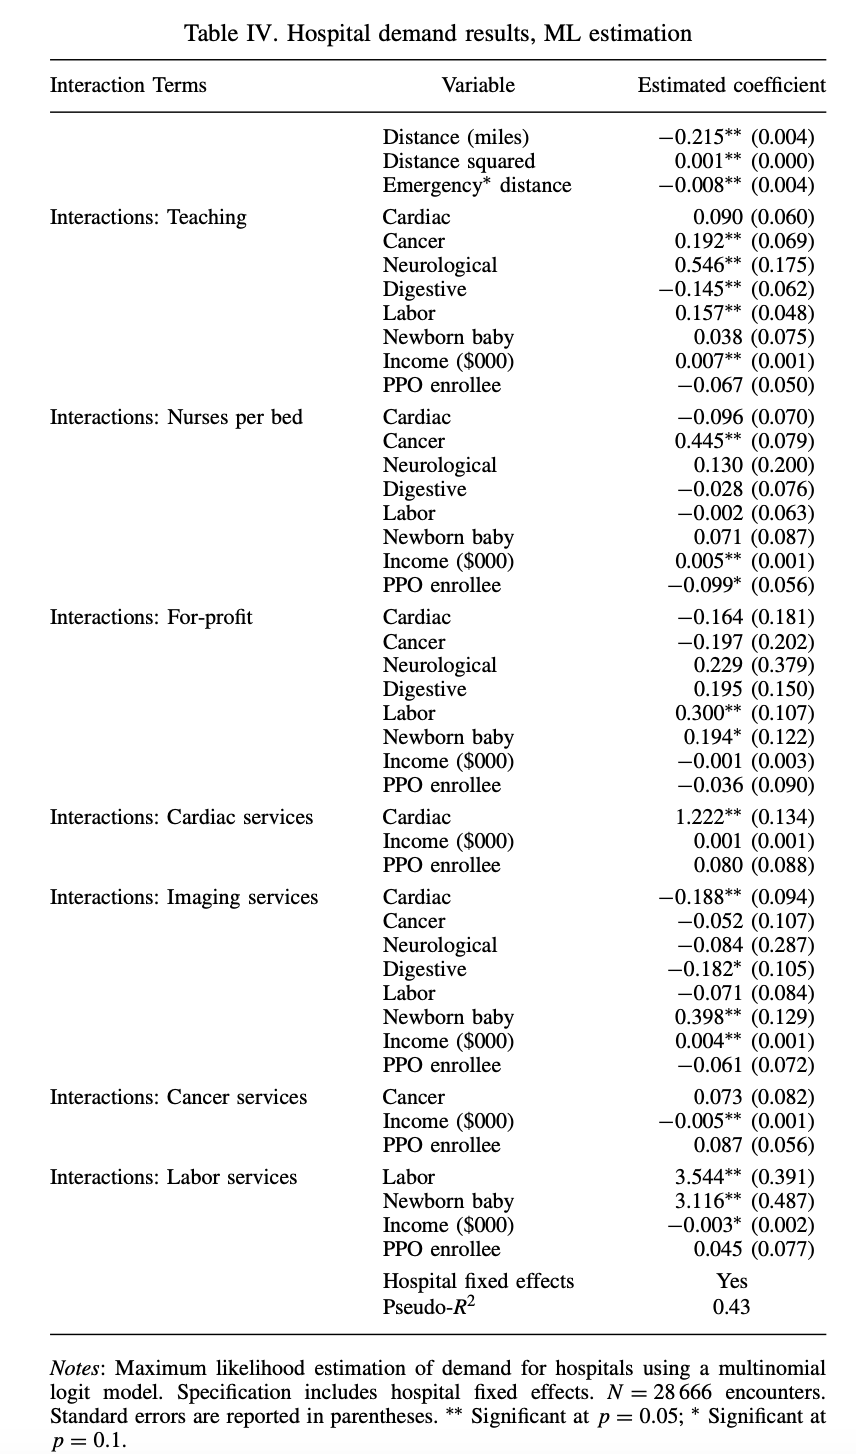
\includegraphics[height=\textheight]{resources/ho_2006}      
% \end{column}
% \begin{column}{0.7\textwidth}
% \begin{itemize}
% \item This just MLE on the full individual data from Ho (2006)
% \begin{itemize}
% \item There is no unobserved heterogeneity, just a deterministic $\beta(y_i)$ where $y_i$ are demographics.
% \end{itemize}
% \item The ``FTC model'' (Raval, Rosenbaum, Wilson RJE 2022)/ (Raval, Rosenbaum, Tenn EI 2017) groups individuals by income, diagnosis, and zip code and estimates a separate set of $\beta_{g(i)}$ for each group.
% \item Hopsitals are a bit special: distance $x_{ij}$ does much of the work (special regressor)
% \item Price endogeneity not really a concern (?)
% \end{itemize}
% \end{column}
% \end{columns}
% \end{frame}

% \begin{frame}{Semiparametric Extensions: Fox Kim Ryan Bajari (QE 2011)}
% \vspace{-0.5cm}
% \begin{align*}
% \nonumber \min_{\pi_i} \sum_{j,t} \left(\mathcal{S}_{jt}(\mathbf{x_t}) - \sum_i \pi_i \cdot s^{*}_{ijt}(\beta^{*}_i, \mathbf{x_t})\right)^2 &
% \quad \text{subject to} \quad s^{*}_{ijt}(\beta^{*}_i, \mathbf{x_t}) = \frac{e^{\beta^{*}_i x_{jt} }}{1+\sum_{j'}e^{\beta^{*}_i x_{j't}}}\\
%    0\leq  \pi_i \leq 1,& \quad   \sum_i \pi_i = 1
% \end{align*}
% \vspace{-0.5cm}
% \begin{enumerate} 
%     \item Draw a large number (thousands?) of $(\beta^{*}_i$ from a prior distribution $g(\beta_i)$ more dispersed than the true $f(\beta_i)$
%     \item Compute individual choice probabilities $ s^{*}_{ijt}(\beta^{*}_i)$
%     \item Estimate above by constrained least squares (non-negative lasso)
%     \item This produces sparse models. (most $\pi_i=0$)
% \end{enumerate}
% Fixed coefficients require EM. See Heiss, Hetzenecker, Osterhaus (JE 2022) for details (and elastic net variant $\sum_i \pi_i^2 \leq t$).
% \end{frame}


% \begin{frame}{Applications of Fixed Grid Estimators}
% These estimators are helpful when computing choice probabilities is time-consuming (ie: when choices are dynamic). Some recent examples:
% \begin{itemize}
%     \item Nevo, Turner, Williams (ECMA 2016): Broadband competition
%     \item Blundell, Gowrisankaran, Langer (AER 2020): EPA regulation
% \end{itemize}
% \end{frame}







% % \begin{frame}

% % \end{frame}


% % \begin{frame}
% % \frametitle{Multinomial Logit: Estimation with Aggregate Data}
% % Now suppose we have aggregate data: $(q_1,\ldots,q_J,q_0)$ where $M = \sum_{j \in \mathcal{J}} q_j$.
% % \begin{itemize}
% % \item If $M$ gets large enough then $(\frac{q_1}{M},\ldots,\frac{q_J}{M},\frac{q_0}{M})\rightarrow (\mathfrak{s}_1,\ldots,\mathfrak{s}_J,\mathfrak{s}_0)$
% % \begin{itemize}
% % \item Idea: Observe $(\mathfrak{s}_1(\mathbf{x_i}),\ldots,\mathfrak{s}_J(\mathbf{x_i}), \mathfrak{s}_0(\mathbf{x_i}))$ without sampling variance.
% % \end{itemize}
% % \item Choose $\theta$ that minimizes distance: MLE? MSM? Least Squares? etc.
% % \end{itemize}
% % \end{frame}

\begin{frame}{Organization}
    \begin{description}
        \item[Past] Lots of good ideas in ``original'' BLP95/99; including some key ones that got ignored and hopefully rediscovered.
        \begin{itemize}
            \item BLP was at its core about \alert{simultaneous supply and demand}.
            \item Much like Chamberlain (1987) the section on optimal IV was ahead of its time.
        \end{itemize}
        \item[Present] Data and Computers are way better than in 1995
        \begin{itemize}
            \item Especially \alert{Micro Data}/ Mini case study
            \item Trying to cram everything in the BLP box is not always the best idea. 
            \begin{itemize}
                \item Some BLP alternatives: analytic inverses, approximations, etc.
            \end{itemize}
        \end{itemize}
        \item[Future] Can we realize the dream of \alert{non-parametric identification} in \alert{estimation}?
            \begin{itemize}
                \item Doing ML not just measuring its impact!
            \end{itemize}
    \end{description}
\end{frame}


\section*{The``Classics'' \#1: Supply Side}

\begin{frame}
\frametitle{Supply Side}
\small
Consider the multi-product Bertrand FOCs where $\arg \max_{p \in \mathcal{J}_f} \pi_f (\mathbf{p})$:
{\begin{align*}
\pi_f (\mathbf{p}) &\equiv \sum_{j \in \mathcal{J}_f} (p_j - c_j) \cdot \sigma_j(\mathbf{p}) + \sum_{k \in \mathcal{J}_g} (p_k - c_k) \cdot \sigma_k(\mathbf{p}) \\
\rightarrow 0&= \sigma_j(\mathbf{p}) + \sum_{k \in \mathcal{J}_f} (p_k - c_k) \frac{\partial \sigma_{k}}{\partial p_j}(\mathbf{p}) 
\end{align*}
}
It is helpful to define the \alert{cross derviative matrix} $\Delta_{(j,k)}(\mathbf{p})  = - \frac{\partial \sigma_{j}}{\partial p_k}(\mathbf{p})$, and the \alert{ownership matrix}:
\begin{align*}
\mathcal{H}_{(j,k)} = \left\{\begin{array}{lr}
          1 & \text{for }  (j,k) \in \mathcal{J}_f \text{ for any } f \\ 
      0 & \text{o.w}\\
        \end{array} \right\}
\end{align*}
We can re-write the FOC in matrix form where $\odot$ denotes Hadamard product (element-wise):
\begin{align*}
        \boldsymbol{\sigma}(\mathbf{p}) &= (\mathcal{H} \odot \Delta(\mathbf{p})) \cdot (\mathbf{p} - \mathbf{mc}), \\
       \mathbf{p}-\mathbf{mc} &=  \underbrace{(\mathcal{H} \odot \Delta(\mathbf{p}))^{-1} \boldsymbol{\sigma}(\mathbf{p})}_{\eta(\mathbf{p},\boldsymbol{\sigma},\theta_2)}.
\end{align*}
\end{frame}


\begin{frame}{What's the point?}
\begin{align*}
p_j &= \underbrace{\frac{1}{1+1/\epsilon_{jj}(\mathbf{p})}}_{\text{Markup}} \left[c_j + \underbrace{\sum_{k \in \mathcal{J}_{f} \setminus j}  (p_k-c_k) \cdot  D_{jk} (\mathbf{p}) }_{\text{opportunity cost}}\right]
\end{align*}
Demand systems have two main deliverables:
\begin{itemize}
\item Own-price elasticities $\epsilon_{jj}(\mathbf{p})$
\item Substitution patterns
\begin{itemize}
\item Cross elasticities: $\epsilon_{jk}(\mathbf{p}) = \frac{p_j}{q_k} \cdot \frac{\partial q_k}{\partial p_j}$
\item Diversion Ratios: $D_{jk}(\mathbf{p}) = \frac{\partial q_k}{\partial p_j}/|\frac{\partial q_j}{\partial p_j}|$
\end{itemize}
\item Other checks: $D_{j0}(\mathbf{p})$ diversion to outside good; $\epsilon^{agg}$ category elasticity to 1\% tax.
\end{itemize}
We did Nash-in-Prices because it is popular but we could have done something else.
\end{frame}









\begin{frame}{Constructing Supply Moments}
If we are willing to impose $MR = MC$ (as in the original BLP papers) we can recover implied markups/ marginal costs:
\begin{align*}
\mathbf{mc}(\theta_2)&\equiv \mathbf{p}- \boldsymbol{\eta}(\mathcal{S}_t,\mathbf{p}_t,\chi_t, y_t, ;\theta_2) \\
f\left(\mathbf{p}- \boldsymbol{\eta}(\mathcal{S}_t,\mathbf{p}_t,\chi_t, y_t, ;\theta_2)  \right) &= [\textrm{x}_{jt} \,, \textrm{w}_{jt}] \theta_3 + \alert{g(q_{jt})} +  \omega_{jt}
\end{align*}
% Which we can solve for $\omega_{jt}$:
% \begin{align*}
% \omega_{jt} &=  f(\mathbf{p}- \boldsymbol{\eta}(\mathbf{p},\mathbf{s},\theta_2) ) -[\textrm{x}_{jt} \,, \textrm{w}_{jt}] \theta_3 
% \end{align*}
\begin{itemize}
\item $f(\cdot)$ is usually $\log(\cdot)$ or identity; it is actually a \alert{production function}
\item $g(q_{jt})$ captures \alert{returns to scale} and requires an additional \alert{instrument}
% \item We can just stack these up with the demand moments $E[\xi_{jt}' Z_{jt}^d]=0$.
%\item Now I have $\dim(Z^d) + \dim(Z^s)$ moments altogether.
% \item This step is optional but can aid in identification (if you believe it).
\end{itemize}
\end{frame}

\begin{frame}{Simultaneous Supply and Demand}
\begin{align*}
\sigma_j^{-1}(\mathcal{S}_t,\mathbf{p}_t,\chi_t, y_t; \theta_2) &= [\mathrm{x}_{jt} \,,  \mathrm{v}_{jt}]\, \theta_1 - \alpha p_{jt} + \xi_{jt}\\
f\left(p_{jt}- \eta_{jt}(\mathcal{S}_t,\mathbf{p}_t,\chi_t, y_t ;\theta_2)  \right) &= [\mathrm{x}_{jt} \,, \mathrm{w}_{jt}]\, \theta_3 +  \omega_{jt}
\end{align*}
We can now form two sets of moments: $\E[\omega_{jt} \mid  z_{jt}^{s}]=0$ and $\E[\xi_{jt} \mid  z_{jt}^{d}]=0$
\begin{itemize}
    \item These provide \alert{overidentifying restrictions} for $(\theta_2, \alpha)$
     \item Conditional on $\theta_2$ (distribution of random coefficients) and $\alpha$ this is just linear IV-GMM again.
     \item The derivatives $\left(\frac{\partial \xi_{jt}}{\partial \theta_2}, \frac{\partial \omega_{jt}}{\partial \theta_2} \right)$ beacuse of $\frac{\partial \eta_{jt}}{\partial \theta_2}$ in particular, are complicated (But \texttt{PyBLP} knows how to do these).
     \item As Steve has made clear this is likely a \alert{many weak IV} situation many potential IV's\\
      (others $x_{-j},w_{-j},v_{-j},y_t$), but hard to know which are strong.
\end{itemize}
\end{frame}


\section*{The``Classics''\#2: Optimal IV}

\begin{frame}{Optimal Instruments (Chamberlain 1987)}
Chamberlain (1987) asks how can we choose $f(z_i)$ to obtain the semi-parametric efficiency bound with conditional moment restrictions:
\begin{align*}
\mathbb{E}[g(z_i,\theta) | z_i]=0 \Rightarrow \mathbb{E}[g(z_i,\theta) \cdot f(z_i) ]=0 
\end{align*}
Recall that the asymptotic GMM variance depends on $(G'\, \Omega^{-1} G\,)$

The answer is to choose instruments related to the (expected) Jacobian of moment conditions w.r.t $\theta$. The true Jacobian at $\theta_0$ is \alert{infeasible}:
\begin{align*}
G=\mathbb{E}\left[\frac{\partial g(z_i,\theta)}{\partial \theta} | z_i, \theta_0 \right]
\end{align*}
Problems: we don't know $\theta_0$ and endogeneity.
%Dominguez and Lobato (2004) point out we can get unlucky and choose an $f(z_i)$ such that $\theta$ is no longer identified(!)
\end{frame}

\begin{frame}{Chamberlain (1987)}
Chamberlain (1987) showed that the approximation to the optimal instruments are given by the expected Jacobian contribution for each observation $(j,t)$: $\mathbb{E}[G_{jt}(\mathbf{Z_t})\, \Omega_{jt}^{-1} | \mathbf{Z_t}]$. For BLP this amounts to:
\begin{align*}
    G&=\mathbb{E}\left[
    \left(\frac{\partial \xi_{jt}}{\partial \theta}, \,
    \frac{\partial \omega_{jt}}{\partial \theta} \right)
| \mathbf{Z_t} \right], \quad 
\Omega = \mathbb{E}\left[
\begin{pmatrix}
    \xi_{jt} \\
    \omega_{jt}
\end{pmatrix}
\begin{pmatrix}
    \xi_{jt}\, \,
    \omega_{jt}
\end{pmatrix}
| \mathbf{Z_t} \right] \\
\xi_{jt} &= \sigma_j^{-1}(\cdot, \theta_2) - [\mathrm{x}_{jt} \,,  \mathrm{v}_{jt}]\, \theta_1 + \alpha p_{jt}\\
\omega_{jt} &= f\left(p_{jt}- \eta_{jt}(\cdot, \theta_2)  \right) -[\mathrm{x}_{jt} \,, \mathrm{w}_{jt}]\, \theta_3 
\end{align*}
For the exogenous variables: $\E\left[\frac{\partial \xi_{jt}}{\partial \theta_1} \mid  z_{jt}^{d} \right]=[\mathrm{x}_{jt} \,,  \mathrm{v}_{jt}]$ and
$\E\left[\frac{\partial \omega_{jt}}{\partial \theta_3} \mid  z_{jt}^{s} \right]=[\mathrm{x}_{jt} \,,  \mathrm{w}_{jt}]$.\\
For the endogenous prices: $\E\left[\frac{\partial \xi_{jt}}{\partial \alpha} \mid  z_{jt}^{d} \right]=\E[p_{jt} \mid z_{jt}^d]$ and
$\E\left[\frac{\partial \omega_{jt}}{\partial \alpha} \mid  z_{jt}^{s} \right]=\E[f'(\cdot) (p_{jt} - \frac{\partial \eta_{jt}}{\partial \alpha}) \mid z_{jt}^s]$.
For the endogenous $\theta_2$: $\mathbb{E}\left[\frac{\partial \boldsymbol{\xi}_{t}}{\partial \theta_2} \mid \mathbf{z_{t}^d} \right] 
=\mathbb{E}\left[\left[\frac{\partial \boldsymbol{\sigma}_{t}}{\partial \boldsymbol{\xi}_t}\right]^{-1} 
\left[\frac{\partial \boldsymbol{\sigma}_{t}}{\partial \theta_2}\right] \mid \mathbf{z_{t}^d} \right]$ and $\mathbb{E}\left[\frac{\partial \omega_{jt}}{\partial \theta_2} \mid \mathbf{z_{t}^s} \right]$\\ (but you can't condition on $p_{jt}$)
\end{frame}


\begin{frame}{Optimal Instruments}
Even with an intitial guess of $\widehat{\theta}$, we still have that $p_{jt}$ or $\eta_{jt}$ depends on $(\omega_{j},\xi_{t})$ in a highly nonlinear way (no explicit solution!). But we have some options:
\begin{itemize}
\item Pray to the God of Sieves:
\begin{itemize}
\item Since any $f(x,z)$ satisfies our orthogonality condition, we can try to choose $f(x,z)$ as a \alert{basis} to approximate optimal instruments. (Newey 1990)
\item This is challenging in practice -- and in fact suffers from a curse of dimensionality.
\item This is frequently given as a rationale behind higher order $x$'s.
\end{itemize}
\item Plug in a guess for \alert{first stage} $p_{jt}$:
\begin{itemize}
\item Reynaert Verboven (2014) suggest $\E[p_{jt} \mid \mathrm{x}_{jt}, \mathrm{w}_{jt}]=mc_{jt}$ (perfect competition), but might as well include other $z_{jt}^d$ (like BLP instruments).
\item $\E[p_{jt} \mid z_{jt}^d]$ is easy, and non-parametric regression is pretty good.
\end{itemize}
\item Use the nonlinearity in the model! (BLP 199)
\end{itemize}
\end{frame}



% \begin{frame}{Optimal Instruments}
% The main challenges:
% \begin{enumerate}
% \item We need an initial estimate of $\widehat{\theta}$
% \item 
% \end{enumerate}
% Potential Solutions
% \begin{enumerate}
% \item Plug in for $E[p_{jt} \mid z_{jt}^d]$.
% \begin{itemize}
% \item Since any $f(x,z)$ satisfies our orthogonality condition, we can try to choose $f(x,z)$ as a \alert{basis} to approximate optimal instruments. (Newey 1990)
% \item This is challenging in practice -- and in fact suffers from a curse of dimensionality.
% \item This is frequently given as a rationale behind higher order $x$'s.
% \item When the dimension of $x$ is low -- this may still be feasible. ($K \leq 3)$.
% \end{itemize}
% \begin{enumerate}
% \end{enumerate}

% \item $p_{jt}$ or $\eta_{jt}$ depends on $(\omega_{j},\xi_{t})$ in a highly nonlinear way (no explicit solution!).
% \end{enumerate}

% \end{frame}


\begin{frame}{Feasible Recipe (BLP 1999)}
\begin{enumerate}
\item Fix $\widehat{\theta}=(\widehat{\theta}_1,\widehat{\theta}_2,\widehat{\theta}_3)$ and draw $(\boldsymbol{\xi}^{*},\boldsymbol{\omega}^{*})$ from empirical density
\item Solve firm FOC's for $\mathbf{\hat{p}_{t}}(\boldsymbol{\xi}^{*},\boldsymbol{\omega}^{*},\widehat{\theta})$ and shares $\mathbf{s_{t}}(\mathbf{\hat{p}_{t}},\widehat{\theta})$
\item Compute necessary Jacobian
\item Average over multiple values of$(\boldsymbol{\xi}^{*},\boldsymbol{\omega}^{*})$. (Lazy approach: use only $(\boldsymbol{\xi}^{*},\boldsymbol{\omega}^{*})=0$).
\end{enumerate}
In simulation the ``lazy'' approach does just as well.\\

 Alternative: Can we use $\mathbb{E}[ \mathbf{p_t} \mid \mathbf{Z_t}]$ instead for (2) if we don't have supply side
\end{frame}



% \begin{frame}{Simplified Version: Reynaert Verboven (2014)}
% \begin{itemize}
% \footnotesize
% \item Optimal instruments are easier to work out if $p = mc$.
% \begin{eqnarray*}
% c = p  + \underbrace{\Delta^{-1} s}_{\rightarrow 0}  = X \gamma_1 + W \gamma_2 + \omega
% \end{eqnarray*}
% \item Linear cost function means linear reduced-form price function (could do nonlinear regression too)
% \begin{eqnarray*}
% E\left[ \frac{\partial \xi_{jt} }{\partial \alpha} | z_t \right] &=& E[p_{jt} | z_t] = x_{jt} \gamma_1 + w_{jt} \gamma_2\\
% E\left[ \frac{\partial \omega_{jt} }{\partial \alpha} | z_t \right] &=& 0 , \quad E\left[ \frac{\partial \omega_{jt} }{\partial \widetilde{\theta}_2} | z_t \right] = 0\\
% E\left[ \frac{\partial \xi_{jt} }{\partial \widetilde{\theta}_2} | z_t \right] &=&E\left[ \frac{\partial \delta_{jt} }{\partial \widetilde{\theta}_2} | z_t \right]\\
% \end{eqnarray*}
% \item If we are worried about endogenous oligopoly markups is this a reasonable idea?
% \item Turns out that the important piece tends to be \alert{shape} of jacobian for $\sigma_x$.
% \item In either case what we care about is $\mathbb{E}[p \mid x, z]$ (the \alert{first stage}). Nothing is free here !
% \end{itemize}
% \end{frame}

% \begin{frame}{Optimal Instruments: Reynaert Verboven (2014)}
% \begin{center}
% \includegraphics[height=0.9\textheight]{resources/verboven.png}
% \end{center}
% \end{frame}


\begin{frame}{IV Comparison: Conlon and Gortmaker (2020)}
\begin{center}
\includegraphics[width=4.9in]{resources/inst_table.png}
\end{center}
\end{frame}

\begin{frame}{IV Comparison: Conlon and Gortmaker (2020)}
\begin{center}
\includegraphics[width=3.9in]{resources/fixed_parameters_simple_plot.pdf}
\end{center}
\end{frame}


\begin{frame}{Cost Shifters Really Matter Conlon Gortmaker (2020)}
\begin{center}
    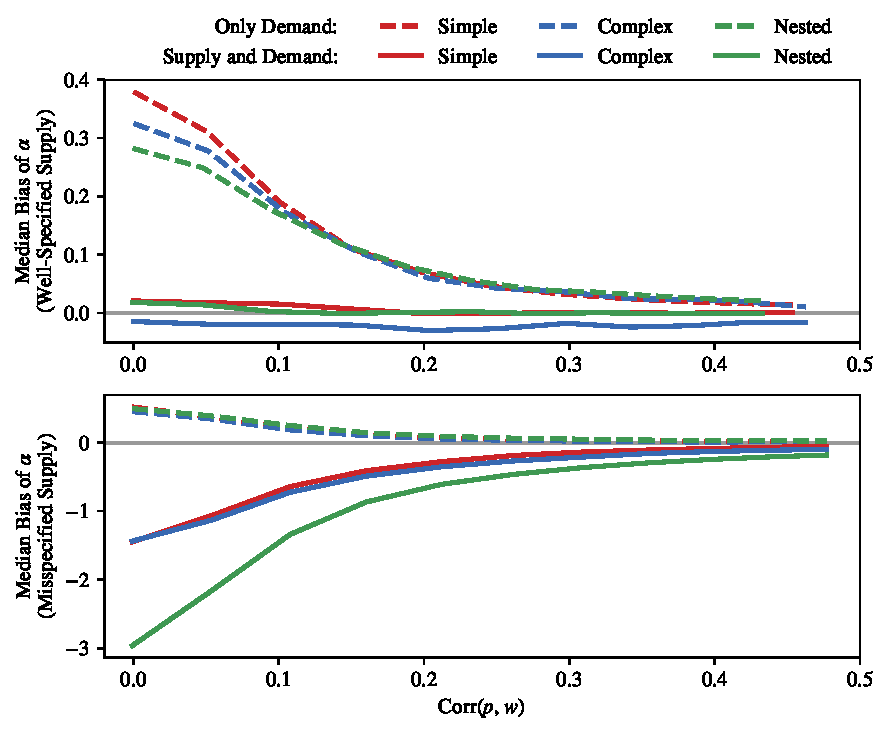
\includegraphics[height=0.95\textheight]{./resources/strength_blp_approximate_bias_alpha_plot.pdf}
\end{center}
\end{frame}

\begin{frame}{Aside: Optimal IV Everywhere! (Backus, Conlon, Sinkinson)}
In our paper on testing conduct we are interested in testing $H_0: \tau=1$ and $H_a: \tau_=0$
\begin{align*}
\omega_{jt} = p_{jt} -\tau \cdot \eta_{jt}^{(a)} - (1-\tau) \cdot \eta_{jt}^{(b)} - h(\textrm{x}_{jt},\textrm{w}_{jt}; \theta_3) 
\end{align*}
The key to the test is to realize that optimal IV: $\E\left[\frac{\partial \omega_{jt}}{\partial \tau} \mid z_{jt}^s \right] = \E\left[\eta_{jt}^{(a)} -\eta_{jt}^{(b)} \mid z_{jt}^s \right]$.
\begin{itemize}
    \item Instruments \alert{predict the difference in markups}!
    \item Can run one non-parametric regression for  $\E\left[\eta_{jt}^{(a)} -\eta_{jt}^{(b)} \mid z_{jt}^s \right]$ and another for the nuisance function (observed markup shifters) $h(\cdot)$.
    \item This is an easy way to do Berry Haile (2014). Duarte, Magnolfi, Sølvsten, Sullivan (2024) get a similar expression with a different approach.
\end{itemize}
\end{frame}


\begin{frame}{Takeaway}
What does this mean:
\begin{itemize}
    \item Optimal IV aren't magic, you probably need good cost shifters.
    \item We should always check $\mathbb{E}[\mathbf{p} \mid \mathbf{z}]$ before we do anything else.
    % \item Can use FRAC to figure out where the heterogeneity is, get startingn values
    \item May want to consider adding a supply side (if you're willing to assume for counterfactuals, why not?)
    \item Certainly should do \texttt{results.compute\_optimal\_instruments()} in \texttt{PyBLP}.
\end{itemize}
\end{frame}


\section{BLP Today}


\begin{frame}{The Good News}
BLP today mostly works
\begin{itemize}
    \item There was some concern (see Knittel Metaxoglou 2014) that BLP estimation was a bit ``fragile''
    \item \texttt{PyBLP} knows how to take derivatives, and we spent a lot of time tuning default options: solving for shares, integration rules, optimization, etc.
    \item Most problems people have today are: \alert{too many parameters, not enough instruments} (or really bad ones).
    \item Cross-market variation in number of products, or characteristics of products would also help.
\end{itemize}
\end{frame}

\begin{frame}{The Bad News: Substitution}
Your BLP model probably isn't as flexible as you think (Sorry!)
\begin{itemize}
\item The unrestricted matrix of of $D_{jk}(\mathbf{p})$'s (or elasticities) is $J \times J$ and probably not feasible to estimate directly. $\rightarrow$ need some \alert{dimension reduction}.
\item Logit simply assumes proportional substitution ${D}_{jk}=\frac{s_k}{1-s_{j}}$ so that $\mathbf{D}(\mathbf{p})$ is of rank one!
\item The BLP solution is to project $\mathbf{D}(\mathbf{p})$ onto a lower-dimensional basis of $x_{j}$ characteristics.
\begin{itemize}
\item Ultimately the basis will be only as good as the characteristics $x_{jt}$ with heterogeneous coefficients.
\item Distributional assumptions on $f(\beta_i)$ (ie: independent normal) further restrict the basis.
\end{itemize}
\item The hardest thing to match is typically \alert{substitution to closest substitutes}.
\begin{itemize}
\item I worry that most BLP models (one RC, etc.) look too much like the plain logit.
\end{itemize}
\item People often assume \alert{HUGE outside good shares} and then have $D_{j0}>0.9$.
\begin{itemize}
    \item We make fun of macro/trade for \alert{monopolistic competition} but easy to estimate something close.
\end{itemize}
\end{itemize}

\end{frame}


\begin{frame}{The Bad News: Elasticities}
If you aren't careful, can still get some weird economics...
\begin{itemize}
\item Plain logit assumes in \alert{elasticities increasing in $p_j$} and \alert{markups that are decreasing}.\\
\begin{itemize}
\item One RC or putting all products in one nest probably isn't going to fix that
\end{itemize}
\item Simple versions tend to lead to \alert{high income} / \alert{price insensitive} consumers buying all the cars, yogurt, etc.
\begin{itemize}
\item $\rightarrow$ Probably everyone should have a \alert{correlated} RC on Price and Constant terms.
\end{itemize}

\item How $f(y_i - \alpha_i p_j)$ looks as it may determine \alert{pass-through}
\\
Griffith, Nesheim O'Connell (2018), Birchall Verboven (2022), Miravete, Seim, Thurk (2023)
\begin{itemize}
\item $\rightarrow$ Lognormal $\alpha_i$ is probably a good idea
\item $\rightarrow$ bins for $\alpha(y_i)$ by income also good (break distributional relationship between $p_{jt}$ and $y_{it}$).
\end{itemize}

\end{itemize}
\end{frame}

\section*{Adding Micro Data}


\begin{frame}{Micro BLP is used a lot: Probably you should use it to.}
    \begin{wideitemize}
        \item Take advantage of much better data available in 2023!
        \item Stack product-level or ``\alert{aggregated}'' moments with ``\alert{micro}'' moments from surveys
        \begin{itemize}
            % \item Impose the \cite{berry1995automobile} share constraint (unlike {\color{light gray}Grieco et al.\ 2023}) \nocite{grieco2023conformant}
            \item Much easier to learn about interactions between demographics and characteristics.
            \item Enables credible \alert{distributional analysis} of policies.
        \end{itemize}
        \item For demographic interactions $\Pi$, you want moments like $Cov(x_j, y_i) = \mathbb{E}[x_j \cdot y_i] -\mathbb{E}[x_j] \cdot \mathbb{E}[y_i]$
        \begin{itemize}
            \item Often easier to construct $\mathbb{E}[x_j \mid y_i]$ or $\mathbb{E}[y_i \mid x_j]$ (often conditional on purchase $j \neq 0$)
        \end{itemize}
        \item For normally distributed $\Sigma$, you want \alert{data on second choices}.
        \begin{itemize}
            \item Original MicroBLP used: $\Cov(x_j, x_{k(\text{-}j)} \,|\, j, k \neq 0)$
        \end{itemize}
        \item The tricky bit is typically working out covariances and weighting matrix\\ $\rightarrow$ this is what Conlon Gortmaker (2023) does! (with help from Myojo \& Kanazawa (2012)).
    \end{wideitemize}
\end{frame}


\begin{frame}{Conlon Gormaker (2023): ``Micro'' \texttt{PyBLP}}
    \vspace{0.5em}
    \scriptsize
    \begin{tabular}{@{\hspace{-1.2em}}r@{\hspace{0.6em}}l@{\hspace{-1.2em}}r@{\hspace{0.6em}}l@{\hspace{-1.2em}}}
        Paper & Micro moments shorthand & Paper & Micro moments shorthand \\
        \midrule
        \cite{petrin2002quantifying} & $\Pr(j \in \mathcal{J} \,|\, i \in \mathcal{I})$, $\E[y_i \,|\, j \in \mathcal{J}]$ & \cite{barwick2017local} & $\Pr(j \in \mathcal{J} \,|\, i \in \mathcal{I})$ \\
        {\color{light gray}Berry et al.\ (2004)} & $\Cov(x_j, y_i \,|\, j \neq 0)$, $\Cov(x_j, x_{k(\text{-}j)} \,|\, j, k \neq 0)$ & \cite{murry2017advertising} & $\E[y_i \,|\, j \in \mathcal{J}]$ \\
        \cite{thomadsen2005effect} & $\Pr(j \in \mathcal{J} \,|\, i \in \mathcal{I})$ & \cite{wollmann2018trucks} & $\E[y_i \,|\, j \in \mathcal{J}]$ \\
        \cite{goeree2008limited} & $\Pr(j \in \mathcal{J} \,|\, i \in \mathcal{I})$ & \cite{li2018better} & $\Pr(j \in \mathcal{J} \,|\, i \in \mathcal{I})$ \\
        \cite{ciliberto2010public} & $\E[y_i \,|\, j \in \mathcal{J}]$ & \cite{li2018empirical} & $\Pr(j \in \mathcal{J} \,|\, i \in \mathcal{I})$ \\
        \cite{nakamura2010accounting} & $\Pr(j \in \mathcal{J} \,|\, i \in \mathcal{I})$ & \cite{backus2021common} & $\E[y_i \,|\, j \in \mathcal{J}]$, $\Cov(x_j, y_i \,|\, j \neq 0)$ \\
        \cite{beresteanu2011gasoline} & $\Pr(j \in \mathcal{J} \,|\, i \in \mathcal{I})$ & \cite{grieco2021evolution} & $\E[x_j \,|\, i \in \mathcal{I}, j \neq 0]$, $\Cov(x_j, x_{k(\text{-}j)} \,|\, j, k \neq 0)$ \\
        \cite{li2012traffic} & $\Pr(j \in \mathcal{J} \,|\, i \in \mathcal{I})$, $\E[y_i \,|\, j \in \mathcal{J}]$ & \cite{neilson2021targeted} & $\E[x_j \,|\, i \in \mathcal{I}, j \neq 0]$ \\
        \cite{copeland2014intertemporal} & $\E[y_i \,|\, j \in \mathcal{J}]$ & \cite{armitage2022regulatory} & $\E[y_i \,|\, j \in \mathcal{J}]$ \\
        \cite{starc2014insurer} & $\Pr(j \in \mathcal{J} \,|\, i \in \mathcal{I})$, $\E[x_j \,|\, i \in \mathcal{I}, j \neq 0]$ & \cite{dopper2022rising} & $\E[y_i \,|\, j \in \mathcal{J}]$ \\
        \cite{ching2015quantifying} & $\Pr(j \in \mathcal{J} \,|\, i \in \mathcal{I})$ & \cite{bodere2023dynamic} & $\Pr(j \in \mathcal{J} \,|\, i \in \mathcal{I})$, $\E[x_j \,|\, i \in \mathcal{I}, j \neq 0]$ \\
        \cite{li2015price} & $\Pr(j \in \mathcal{J} \,|\, i \in \mathcal{I})$ & \cite{montag2023mergers} & $\Cov(x_j, y_i \,|\, j \neq 0)$, $\Cov(x_j, x_{k(\text{-}j)} \,|\, j, k \neq 0)$ \\
        \cite{nurski2016exclusive} & $\E[y_i \,|\, j \in \mathcal{J}]$, $\Cov(x_j, y_i \,|\, j \neq 0)$ & \cite{conlon2023market} & $\E[y_i \,|\, j \in \mathcal{J}]$, $\E[x_j \,|\, i \in \mathcal{I}, j \neq 0]$ \\
        %$\vdots$ & $\vdots$ & $\vdots$ & $\vdots$
    \end{tabular}
    \normalsize
    \vspace{0.5em}
    \begin{wideitemize}
        \item Framework supports most cases we've seen
        \begin{itemize}
            \item Demographic/choice-based sampling, conditioning, covariances, \alert{second choices} $k \neq j$ too!
        \end{itemize}
    \end{wideitemize}
\end{frame}



\begin{frame}{Some words of caution}
    
    \begin{wideitemize}
    \item There are \alert{optimal micro moments} which approximate scores\\ (see Conlon Gortmaker 2023).
        \begin{itemize}
            \item There are no efficiency guarantees for \alert{inconsistent} pilot estimates $\hat{\theta}$
            \item For first step, can use standard moments or score at informed guess of $\theta_0$
        \end{itemize}
        
        \item Most pairs of datasets have at least some  \alert{incompatibilities} in timing, variables, etc.
        \begin{itemize}
            \item Optimal micro moments will only work well if incompatibilities are small
            \item If large, match moments you expect to be compatible, e.g.\ correlations if scales are different
            \item Problem exists for ``typical moments'' in Alcohol:\\
             $\E[Purch \mid  y_{it}]$ vs. $\E[y_{it} \mid Purch]$ when $\E[Purch]$ is \alert{incompatible}.
        \end{itemize}
    
        \item Quadrature behaves poorly with \alert{discontinuities} in moments like ``$\E[x_{jt} \mid y_{it} < \overline{y}, \, j \neq 0]$''
        \begin{itemize}
            \item Instead, use Monte Carlo methods or moments continuous in $y_{it}$ like ``$\Cov(x_{jt}, y_{it} \mid j \neq 0)$''
        \end{itemize}
    \end{wideitemize}
\end{frame}



\begin{frame}{Complete Micro Data: Grieco Murry Pinkse Sagl (2023)}
Like a one-step version of Goolsbee Petrin (2004)
        \begin{align*}
            (\hat{\beta},\hat{\theta}_2,\hat{\delta}) = \arg\min_{\beta,\theta_2,\delta} -\log\hat{L}(\theta_2,\delta)+\hat{\Pi}(\beta,\delta)
        \end{align*}
        \begin{enumerate}
            \item the Mixed Data Likelihood Estimator:
                \begin{align*}
                    \log\hat{L}(\theta,\delta) =\sum_{m=1}^M\sum_{j=0}^{J_m}\sum_{i=1}^{N_m} d_{ijm}(D_{im} \underbrace{\log \pi_{jm}^{y_{im}}(\theta_2,\delta)}_{\text{individual choices}} + (1-D_{im}) \underbrace{\log\pi_{jm}(\theta_2,\delta)}_{\text{aggregate share}})%\\
                     %=\sum_{m=1}^M\sum_{j=0}^{J_m}\sum_{i=1}^{N_m} D_{im} d_{ijm} \log\frac{\pi_{jm}^{y_{im}}}{\pi_{jm}} + \sum_{m=1}^M N_m\sum_{j=0}^{J_m}s_{jm}\log\pi_{jm}
                \end{align*}
        \item including the BLP moment conditions
        \begin{align*}
            \hat{\Pi}(\beta,\delta) = \frac{1}{2}\hat{g}^\intercal(\beta,\delta)\cdot \hat{\mathcal{W}}\cdot\hat{g}(\beta,\delta)
        \end{align*}
        where $\hat{\mathcal{g}}^\intercal(\beta,\delta) = \sum_{m=1}^M \sum_{j=1}^{J_m} z_{jm}(\delta_{jm}-\beta^\intercal x_{jm})$.\\
    \end{enumerate}
    Trick in the paper: getting $\hat{\mathcal{W}}$ correct.
\end{frame}



\section*{Quick Case Studies: Micro Data, Second Choices, Supply}


\begin{frame}\frametitle{Grieco, Murry, Yurukoglu (QJE 2024)}
\begin{columns}
\begin{column}{0.66\textwidth}
     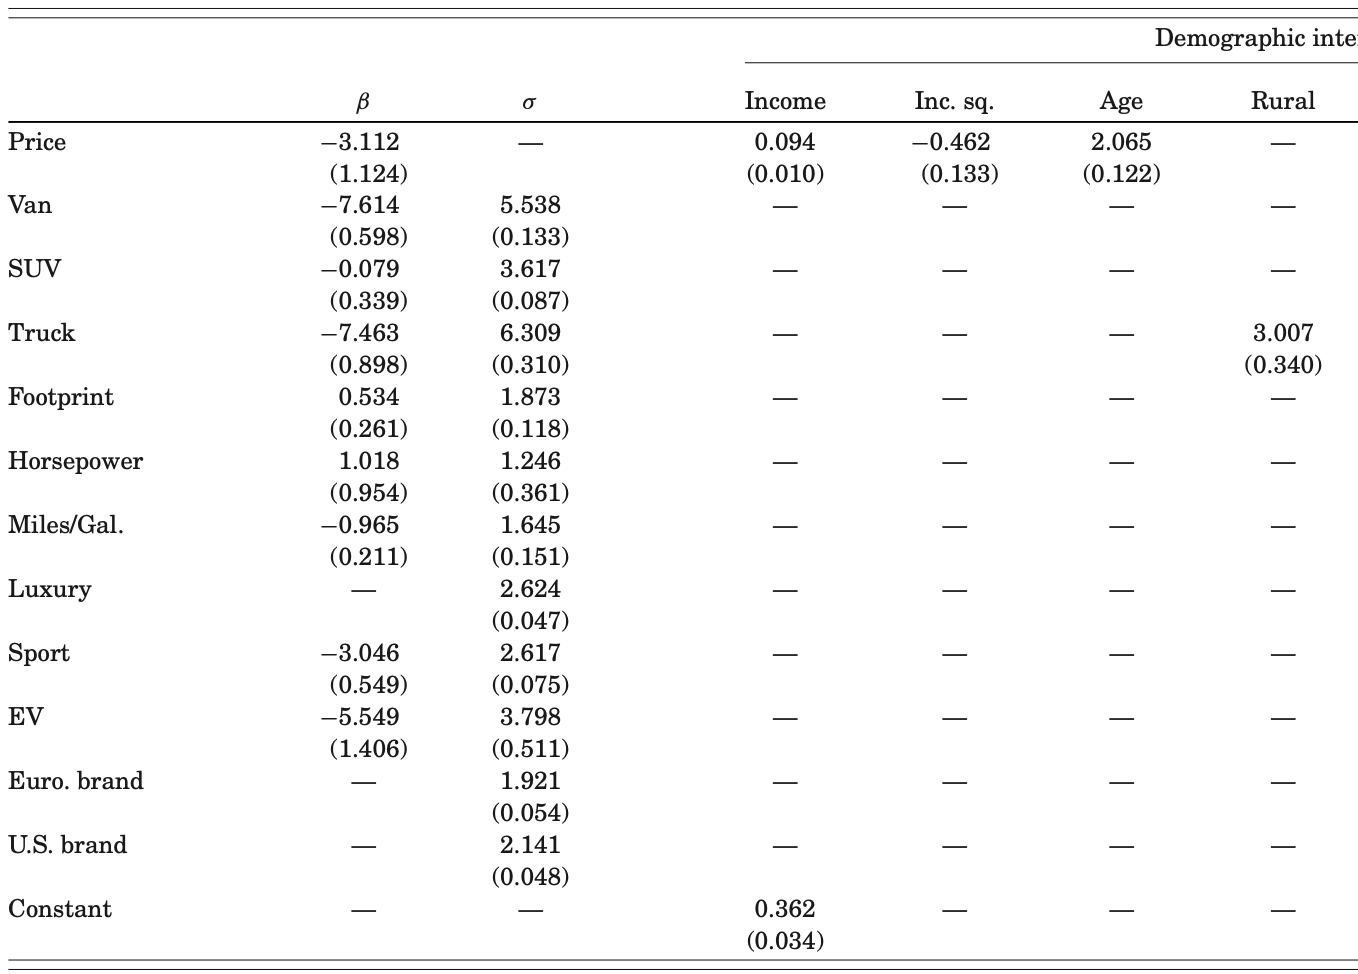
\includegraphics[width=\textwidth]{resources/gmy1}      
\end{column}
\begin{column}{0.33\textwidth}
Best MicroBLP application?
\begin{wideitemize}
\item  Average characteristics by income, age, family size:\\
$\E[x_j \,|\, i \in I, j \neq 0]$
\item Covariance of characteristics for 1st and 2nd choices:\\ $\Cov(x_j, x_{k(\text{-}j)} \,|\, j, k \neq 0)$
\item I would make Price lognormal and put RC on constant...
\end{wideitemize}
\end{column}
\end{columns}
\end{frame}


\begin{frame}{Supply and Micro Data: (Conlon Rao 2023)}
Consumer $i$ chooses product $j$ (brand-size-flavor) in quarter $t$:
\begin{align*}
u_{ijt} &= \beta_{i}^0 -  \alpha_i\, p_{jt} + \beta_i^{1750}\, \cdot \mathbb{I}[1750mL]_j + \gamma_j + \gamma_t+ \varepsilon_{ijt}(\rho)\\
\begin{pmatrix}
\ln \alpha_i\\
\beta_i
\end{pmatrix} &=
\begin{pmatrix}
\overline{\alpha}\\
\theta_1
\end{pmatrix} + \Sigma \cdot \nu_i + \sum_{k} \Pi_k \cdot \mathbb{I}\{LB_k \leq \text{Income}_i < UB_k\} 
\end{align*}
\begin{itemize}
\item Nesting Parameter $\rho$: Substitution within category (Vodka, Gin, etc.) %(Vodka/Tequila/Rum/Gin/Whiskey)
\item Consumers of different income levels have different mean values for coefficients
\item Conditional on income, normally distributed unobserved heterogeneity for:
\begin{itemize}
\item Price $\alpha_i$: \alert{Lognormal}
\item Constant $\beta_{i}^0$ (Overall demand for spirits)
\item Package Size: $\beta_{i}^{1750}$ (Large vs. small bottles)
\end{itemize}
\end{itemize}
\end{frame}


% \begin{frame}{Wholesale Margins Under Post and Hold}
% \begin{columns}[T]
% \begin{column}{.5\textwidth}
% \begin{center}
% 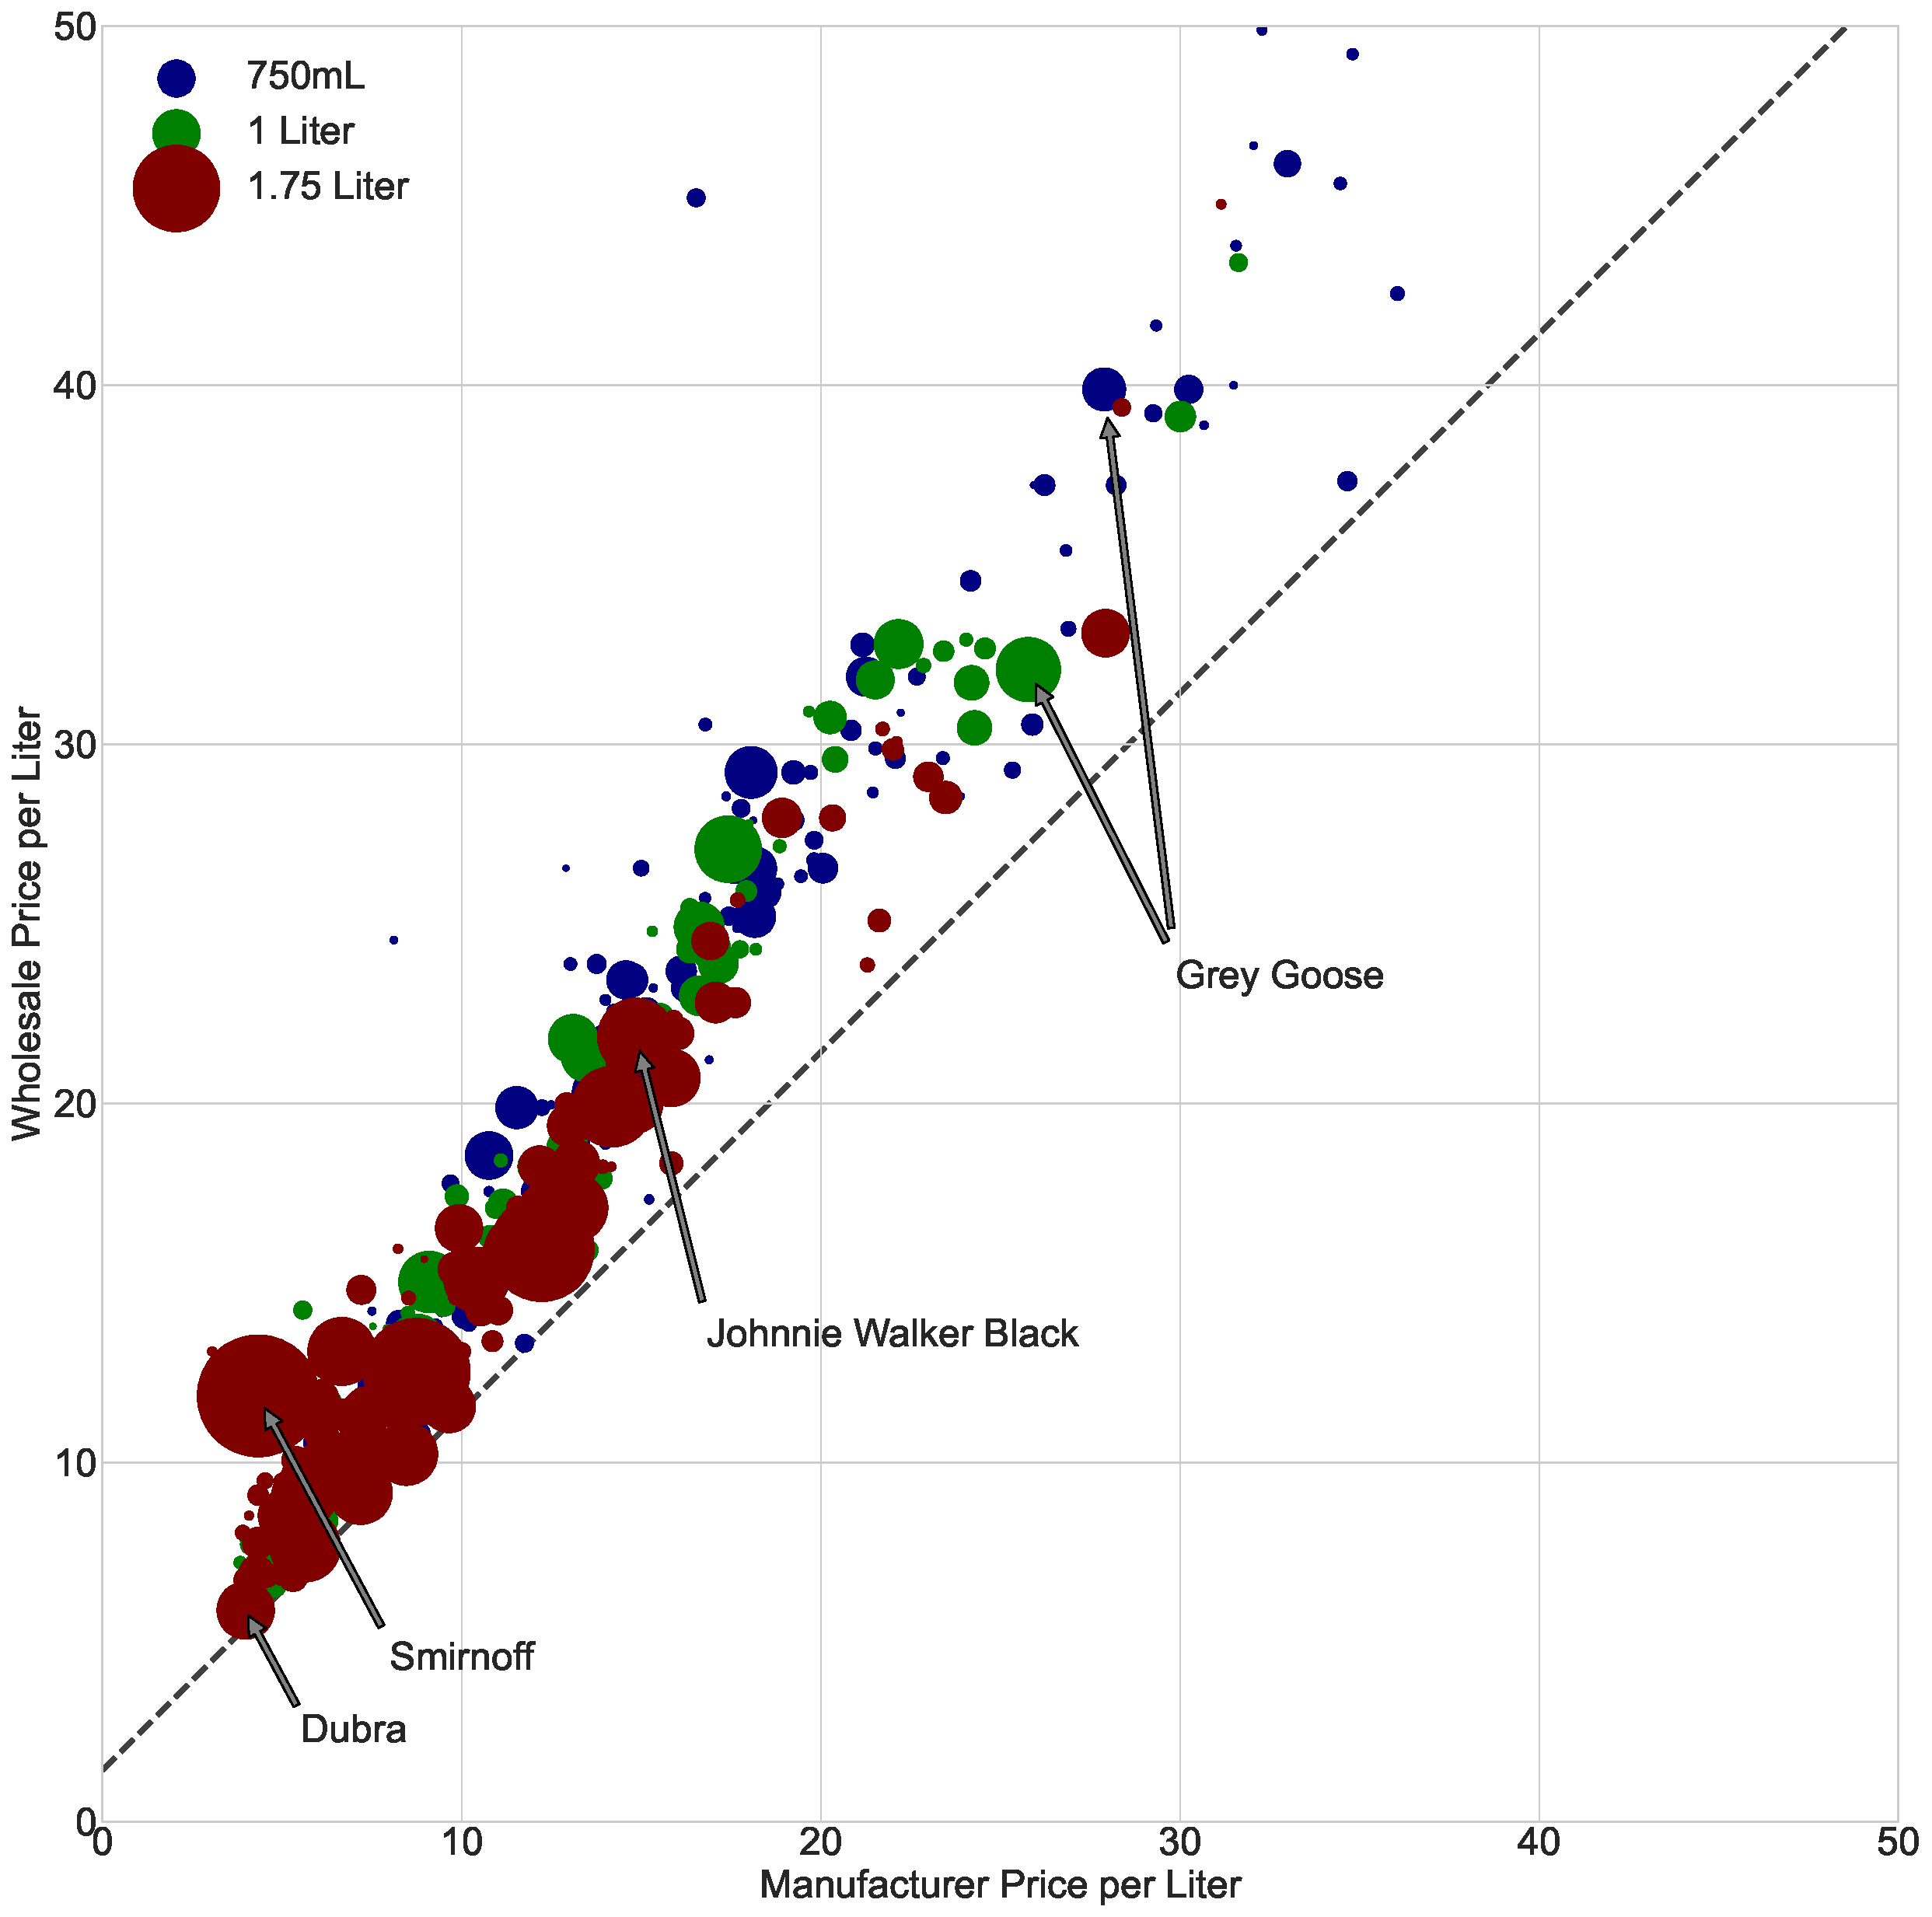
\includegraphics[height=0.88\textheight]{resources/figure4_manuf_wholesale_price.pdf}
% \end{center}
% \end{column}
% \hfill
% \begin{column}{.5\textwidth}
%   \begin{itemize}
%   \item Price Cost Margins (and Lerner Markups) are higher on premium products
%   \item Markups on least expensive products (plastic bottle vodka) are very low.
%   \item Smirnoff (1.75L) is best seller\\ (high markup / outlier).
%   \item A planner seeking to minimize ethanol consumption would flatten these markups!
%   \item Matching this pattern is kind of the whole ballgame !
%   \item Plain logit gives $\epsilon_{jj} = \alpha \cdot p_j  \cdot (1-s_j)$.
%   \end{itemize}
%   \end{column}
% \end{columns}
% \end{frame}



\begin{frame}{Demand Estimates (from \texttt{PyBLP}, Conlon Gortmaker (2020, 2023))}
\begin{columns}[T]
 \hspace{-1.5cm}
 \begin{column}{.68\textwidth}
\vspace{-0.3cm}
    \begin{center}
    \scalebox{0.55}{
    \begin{tabular}{lccc} 
\toprule 
\multicolumn{1}{c}{$\Pi$} &  Const &  Price &  1750mL \\ 
\cmidrule(r){1-1} \cmidrule(rrr){2-4} 
Below \$25k  &  2.928 & -0.260 &   0.543 \\
            &  (0.233) &  (0.056) &   (0.075) \\
\$25k-\$45k   &  0.184 & -0.170 &   0.536 \\
            &  (0.236) &  (0.054) &   (0.083) \\
\$45k-\$70k   &  0.000 & -0.179 &   0.980 \\
            &  (0.000) &  (0.053) &   (0.093) \\
\$70k-\$100k  & -0.452 & -0.496 &   0.608 \\
            &  (0.227) &  (0.051) &   (0.079) \\
Above \$100k & -1.777 & -1.543 &   0.145 \\
            &  (0.234) &  (0.047) &   (0.055) \\
\midrule \multicolumn{1}{c}{$\Sigma^2$}& \multicolumn{2}{c}{} \\ \cmidrule(r){1-1} \cmidrule(rrr){2-4}
Constant    &   1.167 & 0.695   &  \\
            &  (0.236)&(0.048) &   \\
Price       &   0.695 & 0.697  \\
            &   (0.048) &(0.028) \\
\midrule  
\multicolumn{1}{l}{Nesting Parameter $\rho$} &  &0.423&    \\ 
& &(0.026)&     \\ 
\multicolumn{1}{l}{Fixed Effects} &   \multicolumn{3}{c}{Brand+Quarter}\\ 
\midrule 
%\multicolumn{1}{c}{}& \multicolumn{3}{c}{Model Predictions} \\ 
\multicolumn{1}{c}{Model Predictions}& 25\% & 50\% & 75\% \\ \midrule\midrule
Own Elasticity:  $\frac{\partial \log q_j}{\partial \log p_j}$                  & -5.839 & -5.162 & -4.733 \\
Aggregate Elasticity: $\frac{\partial \log Q}{\partial \log P}$            & -0.333 & -0.329 & -0.322 \\
Own Pass-Through: $\frac{\partial p_j}{\partial c_j}$          & 1.256 & 1.284 &  1.320 \\
Observed Wholesale Markup (PH)  &  0.188 &  0.233 &  0.276 \\
Predicted Wholesale Markup (PH) &  0.205 &  0.231 &  0.259 \\
\bottomrule 
\end{tabular}
    }
    \end{center}
  \end{column}
  \hfill
 \hspace{-2.2cm}
\begin{column}{.55\textwidth}
  \begin{itemize}
    \item Demographic Interactions w/ 5 income bins \\ (matched to micro-moments)
    \item Correlated Normal Tastes: (Constant, Large Size, Price)
    \item Supply moments exploit observed upstream prices and tax change (ie: match observed markups).
    \vspace{-0.2cm}
    \begin{align*}
    \mathbb{E}[\omega_{jt}]=0, \text{ with }\omega_{jt} = \left(p^w_{jt}  - p^m_{jt}-\tau_{jt} \right) -\eta_{jt}\left(\theta_2\right).
    \end{align*}
   \vspace{-0.8cm}
    \item Match repeat purchase share within (Vodka, Gin, Rum, etc.) as in Atalay, Frost, Sorensen, Sullivan, and Zhu (2023)
    \item Pass-through consistent with estimates from our AEJ:Policy paper.
  \end{itemize}
\end{column}
\end{columns}
\end{frame}

\begin{frame}{Elasticities and Diversion Ratios}
\begin{center}
    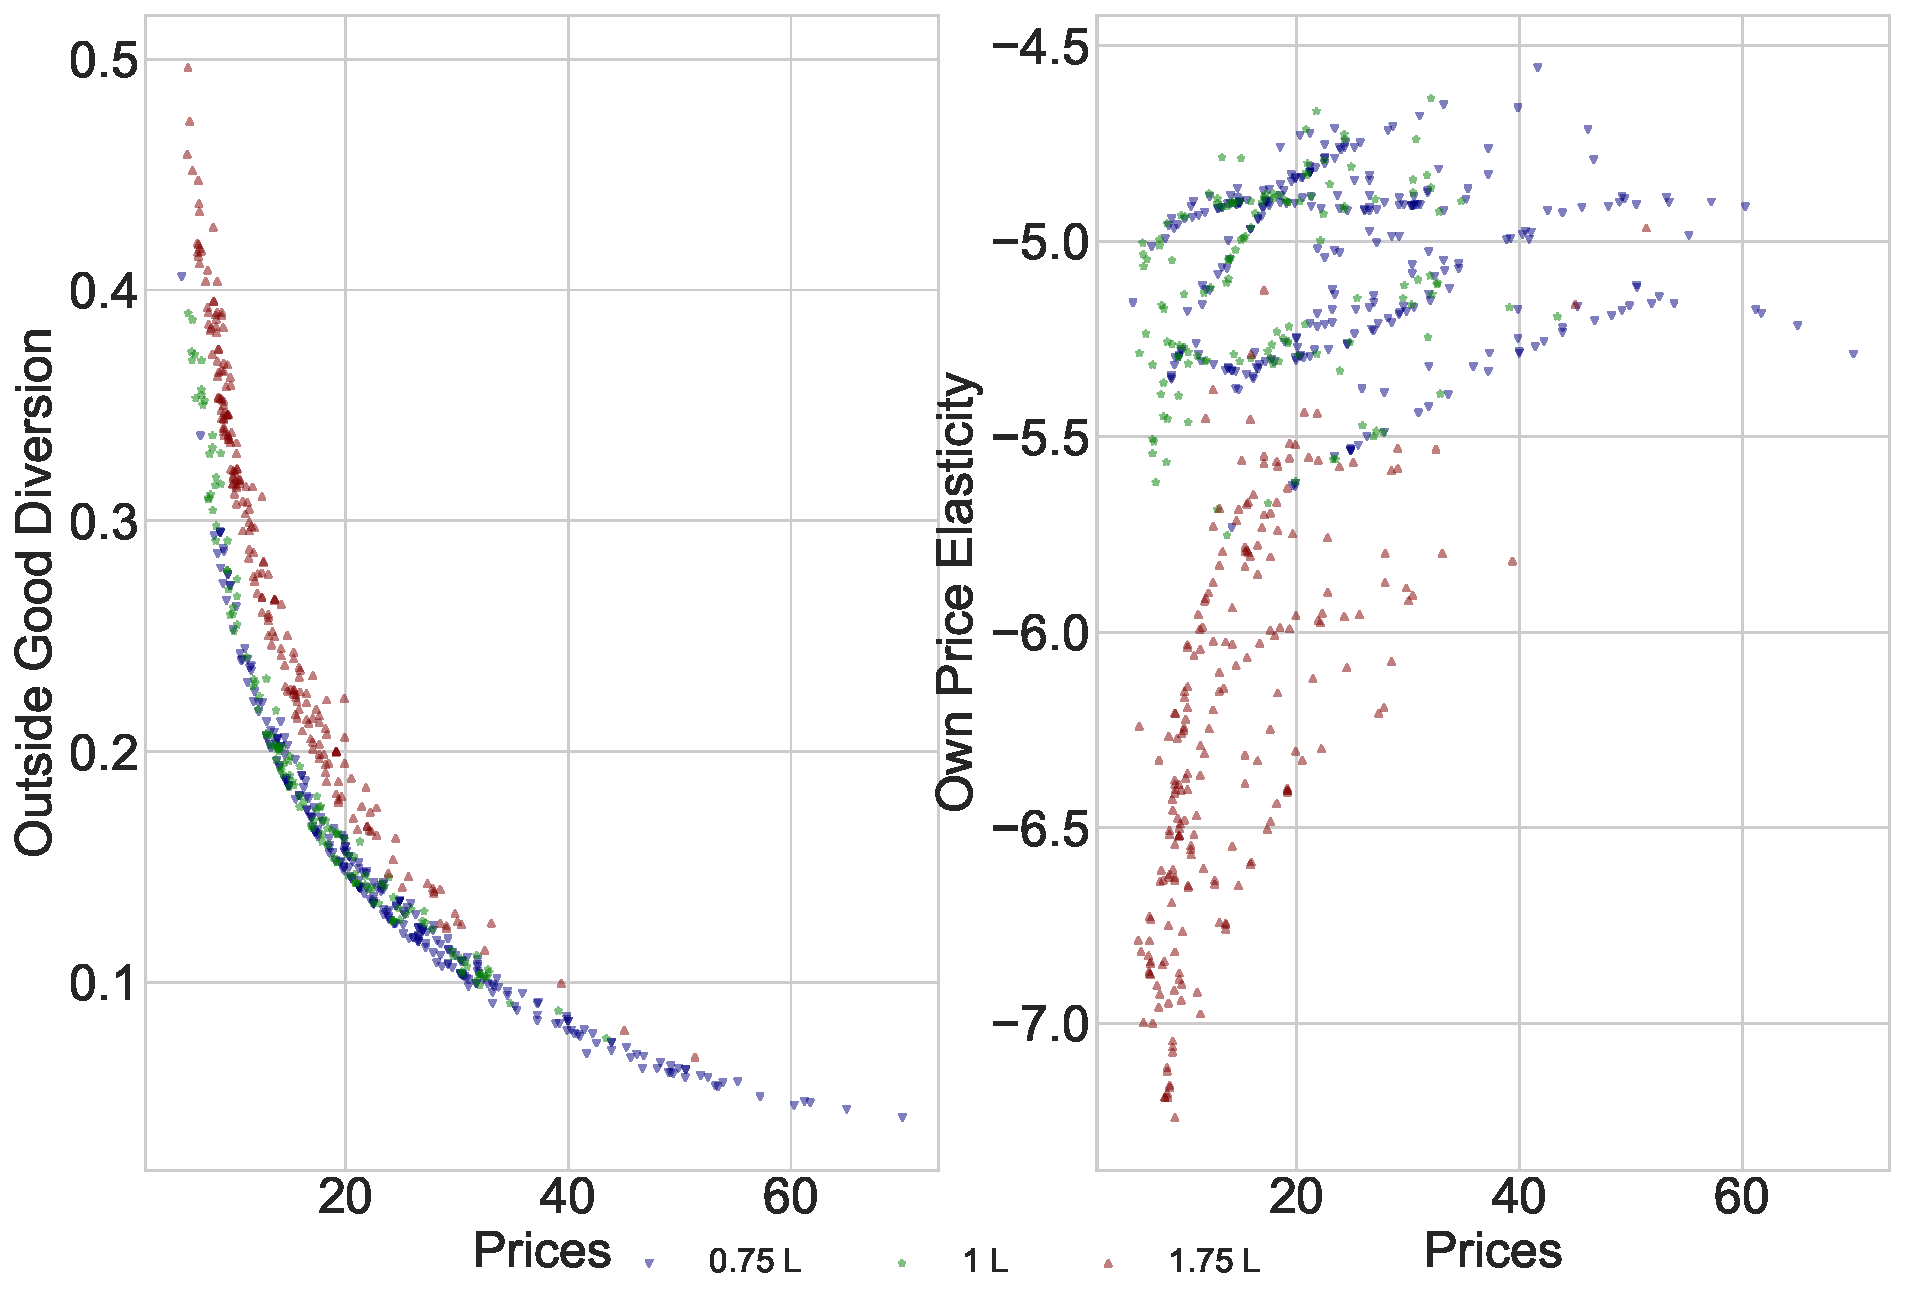
\includegraphics[height=0.95\textheight]{./resources/figure6_outside_diversion_elas_v2.pdf}
\end{center}
\end{frame}



\begin{frame}{Diversion Ratios}
\begin{center}
\scalebox{0.6}{
\begin{tabular}{lrrlrr} 
\toprule 
{}&  Median Price &  \% Substitution &  {}&  Median Price &  \% Substitution \\ 
\midrule 
\multicolumn{1}{c}{Capt Morgan Spiced 1.75 L (\$15.85)} & \multicolumn{5}{c}{ Cuervo Gold 1.75 L (\$18.33) } \\ \cmidrule(lr){1-1} \cmidrule(lrr){4-6} 
\midrule 
        Bacardi Superior Lt Dry Rum 1.75 L & 12.52 & 13.07 &                    Don Julio Silver 1.75 L & 22.81 & 5.00 \\
                   Bacardi Dark Rum 1.75 L & 12.52 &  2.71 &                          Cuervo Gold 1.0 L & 21.32 & 3.82 \\
         Bacardi Superior Lt Dry Rum 1.0 L & 15.03 &  2.44 &              Sauza Giro Tequila Gold 1.0 L &  8.83 & 3.07 \\
                           Smirnoff 1.75 L & 11.85 &  2.36 &                            Smirnoff 1.75 L & 11.85 & 2.44 \\
     Lady Bligh Spiced V Island Rum 1.75 L &  9.43 &  2.18 &                       Absolut Vodka 1.75 L & 15.94 & 2.06 \\
\midrule 
\multicolumn{1}{c}{Woodford 0.75 L (\$34.55)} & \multicolumn{5}{c}{ Beefeater Gin 1.75 L (\$17.09) } \\ \cmidrule(lr){1-1} \cmidrule(lrr){4-6} 
\midrule 
             Jack Daniel Black Label 1.0 L & 27.08 & 7.66 &                           Tanqueray 1.75 L & 17.09 & 12.80 \\
            Jack Daniel Black Label 1.75 L & 21.85 & 4.91 &                             Gordons 1.75 L & 11.19 &  4.14 \\
            Jack Daniel Black Label 0.75 L & 29.21 & 4.83 &                        Seagrams Gin 1.75 L & 10.23 &  2.85 \\
                         Makers Mark 1.0 L & 32.79 & 4.52 &                              Bombay 1.75 L & 21.95 &  2.27 \\
                        Makers Mark 0.75 L & 31.88 & 2.80 &                            Smirnoff 1.75 L & 11.85 &  2.27 \\
\midrule 
\multicolumn{1}{c}{Dubra Vdk Dom 80P 1.75 L (\$5.88)} & \multicolumn{5}{c}{ Belvedere Vodka 0.75 L (\$30.55) } \\ \cmidrule(lr){1-1} \cmidrule(lrr){4-6} 
\midrule 
                        Popov Vodka 1.75 L &  7.66 & 7.56 &                           Grey Goose 1.0 L & 32.08 & 5.09 \\
                           Smirnoff 1.75 L & 11.85 & 3.15 &                       Absolut Vodka 1.75 L & 15.94 & 3.82 \\
                    Sobieski Poland 1.75 L &  9.09 & 3.14 &                        Absolut Vodka 1.0 L & 24.91 & 2.74 \\
                 Grays Peak Vdk Dom 1.75 L &  9.16 & 2.87 &                            Smirnoff 1.75 L & 11.85 & 2.43 \\
                        Wolfschmidt 1.75 L &  6.92 & 2.48 &                          Grey Goose 0.75 L & 39.88 & 2.22 \\
\bottomrule 
\end{tabular}
}
\end{center}
% \begin{tablenotes}
% \item Note: The table above reports diversion rates for five popular products.  Per liter wholesale prices are reported for 2013Q2. We compute the diversion ratio for a small price change $D_{j \rightarrow k} = \frac{\partial q_{k}}{\partial q_{j}}/\left|\frac{\partial q_{j}}{\partial q_{j}}\right|$. Substitutes maintain the same product category but differ across products due to the nesting parameter and random coefficients incorporated in the RCNL model.
% \item A plain logit would predict the best substitute as the product with the largest overall share: Smirnoff Vodka (80 Proof, 1.75L) with $s_{jt} = 1.2\%$ or $4.38\%$ of ``inside'' sales.
% \item Source: Authors' calculations
% \end{tablenotes}
\end{frame}


\section{Approximating the Problem}




\begin{frame}
\frametitle{BLP 1995/1999 and Berry Haile (2014)}
Think about a \alert{generalized inverse} for $\sigma_{j}(\boldsymbol{\delta_{t}}, \mathbf{x}_t,\theta_2) = \mathfrak{s}_{jt}$ so that 
\begin{align*}
%\sigma_{jt}^{-1}(\mathcal{S}_{\cdot t},\widetilde{\theta}_2)+\alpha p_{jt}&= h(x_{jt},v_{jt},\theta_1)   + \xi_{jt}\\
 \sigma_{jt}^{-1}(\mathcal{S}_{\cdot t},\widetilde{\theta}_2)&= \delta_{jt} \equiv x_{jt} \beta -\alpha p_{jt} +  \xi_{jt} 
\end{align*}
 \begin{itemize}
\item After some transformation of data (shares $\mathcal{S}_{\cdot t}$) we get \alert{mean utilities} $\delta_{jt}$.
% \begin{itemize}
% \item We assume $\delta_{jt}=h(x_{jt},v_{jt},\theta_1) -\alpha p_{jt} + \xi_{jt}$ follows some parametric form (often linear).
%  \end{itemize}
\item Same IV-GMM approach after transformation
\item Examples:
\begin{itemize}
\item Plain Logit: $\sigma_{j}^{-1}(\mathcal{S}_{\cdot t}) = \ln \mathfrak{s}_{jt}- \ln \mathfrak{s}_{0t}$
\item Nested Logit: $\sigma_{j}^{-1}(\mathcal{S}_{\cdot t},\rho) = \ln \mathfrak{s}_{jt}- \ln \mathfrak{s}_{0t} - \rho  \ln \mathfrak{s}_{j|gt}$
\item Three level nested logit: $\sigma_{j}^{-1}(\mathcal{S}_{\cdot t},\rho) = \ln \mathfrak{s}_{jt}- \ln \mathfrak{s}_{0t} -\sum_{d=1}^2 \rho_d \ln \left(\frac{\mathfrak{s}_{jt}}{\mathfrak{s}_{d(j), t}}\right)$ (Verboven 1996)
\item IPDL: $\sigma_{j}^{-1}(\mathcal{S}_{\cdot t},\rho) = \ln \mathfrak{s}_{jt}- \ln \mathfrak{s}_{0t}-\mathbf{x}_{j t} \boldsymbol{\beta}-\alpha p_{j t}-\sum_{d=1}^D \rho_d \ln \left(\frac{\mathfrak{s}_{jt}}{\mathfrak{s}_{d(j), t}}\right)+\xi_{j t}$\\ (Fosgerau, Monardo, De Palma (2022))
 \end{itemize}
 \item Anything with a share requires an IV (otherwise $\rho \rightarrow 1$).
 \end{itemize}
\end{frame}



\begin{frame}{Intuition from Linear IV (FRAC: Salanie and Wolak)}
Simple case where $\theta_0 = (\beta_0, \pi_0, \sigma_0)'$. A second-order Taylor expansion around $\pi_0 = \sigma_0 = 0$ gives the following linear model with four regressors:
\begin{align*}
    \log\frac{\mathcal{S}_{jt}}{\mathcal{S}_{0t}} \approx \beta_0 x_{jt} + \pi_0 m_t^y x_{jt} + \left(\sigma_0^2+  \pi_0^2 v_t^y \right) a_{jt} + \xi_{jt}, \quad a_{jt} = \Big(\frac{x_{jt}}{2} - \sum_{k \in \mathcal{J}_t} \alert{\mathcal{S}_{kt}} \cdot x_{kt}\Big) \cdot x_{jt}
\end{align*}
\begin{itemize}
    \item $m_t^y = \sum_{i \in \mathcal{I}_t} w_{it} \cdot y_{it}$ is the within-market demographic mean
    \item $v_t^y = \sum_{i \in \mathcal{I}_t} w_{it} \cdot (y_{it} - m_t^y)^2$ is its variance
    \item $a_{jt}$ is an ``artificial regressor'' that reflects within-market differentiation of the product characteristic $x_{jt}$.\\
    \item Linear but we still need an IV for $a_{jt}$ (\alert{endogenous shares!})
\end{itemize}
Implemented in Julia by Jimbo Brand  \url{https://github.com/jamesbrandecon/FRAC.jl}
% where $m_t^y = \sum_{i \in \mathcal{I}_t} w_{it} \cdot y_{it}$ is the within-market demographic mean, $v_t^y = \sum_{i \in \mathcal{I}_t} w_{it} \cdot (y_{it} - m_t^y)^2$ is its variance, and $a_{jt}$ is an ``artificial regressor'' that reflects within-market differentiation of the product characteristic $x_{jt}$.\footnote{\cite{salanie2019fast} give additional intuition for the functional form of $a_{jt}$. A quadratic form is unsurprising because $x_{jt}$ multiplied $\nu_{it}$. The $\frac{1}{2}$ comes from the symmetric shape of the logistic distribution.} If $\pi_0 = \sigma_0 = 0$, the approximation is exact, and collapses to a simple logit regression: $\log(\mathcal{S}_{jt} / \mathcal{S}_{0t}) = \delta_{jt} = \beta_0 x_{jt} + \xi_{jt}$.
\end{frame}


\begin{frame}{Connection or when do GH IV work well?}
Recall the GH IV are:
\begin{align*}
x_{jt}^2 + \underbrace{\frac{1}{J} \cdot \sum_k x_{kt}^2}_{\text{ constant for } t } - \alert{2 x_{jt}  \cdot \sum_k  \frac{1}{J} \cdot x_{kt}}
\end{align*}
and the artificial regressor is
\begin{align*}
\frac{1}{2} x_{jt}^2 - \alert{2 x_{jt} \cdot \sum_k \mathcal{S}_{kt}  \cdot x_{kt}}
\end{align*}
\begin{itemize}
\item We should be \alert{share weighting} the interaction term, but GH assume equal weighting.\\
\item Should be able to do better than these IV (but ideal is infeasible...)
\item Alternative take: GH propose IIA test that looks a lot like Salanie Wolak estimator. Good for starting values? Or as pre-test for heterogeneity?
\item Warning: I find these are always nearly colinear and run PCA first...
\end{itemize}
\end{frame}






% \begin{frame}{Optimal Instruments (Chamberlain 1987)}
% Chamberlain (1987) asks how can we choose $f(z_i)$ to obtain the semi-parametric efficiency bound with conditional moment restrictions:
% \begin{align*}
% \mathbb{E}[g(z_i,\theta) | z_i]=0 \Rightarrow \mathbb{E}[g(z_i,\theta) \cdot f(z_i) ]=0 
% \end{align*}
% Recall that the asymptotic GMM variance depends on $(G'\, \Omega^{-1} G\,)$

% The answer is to choose instruments related to the (expected) Jacobian of moment conditions w.r.t $\theta$. The true Jacobian at $\theta_0$ is \alert{infeasible}:
% \begin{align*}
% G=\mathbb{E}\left[\frac{\partial g(z_i,\theta)}{\partial \theta} | z_i, \theta_0 \right]
% \end{align*}
% %Dominguez and Lobato (2004) point out we can get unlucky and choose an $f(z_i)$ such that $\theta$ is no longer identified(!)
% \end{frame}


% \begin{frame}{Optimal Instruments (Chamberlain 1987)}
% Consider the simplest IV problem:
% \begin{align*}
% y_i &= \beta x_i + \gamma v_i + u_i \quad \text{ with } \quad \mathbb{E}[u_i | v_i, z_i] =0 \\
% u_i &= \left(y_i - \beta x_i - \gamma v_i \right) \\
% g(x_i,v_i,z_i) &= \left(y_i - \beta x_i - \gamma v_i \right) \cdot [v_i,\, z_i]
%  \end{align*}
%  Which gives:
% \begin{align*}
% \mathbb{E}\left[\frac{\partial g(x_i,v_i, z_i,\theta)}{\partial \gamma} \mid v_i, z_i \right] &\propto v_i\\
% \mathbb{E}\left[\frac{\partial g(x_i,v_i, z_i,\theta)}{\partial \beta} \mid v_i, z_i \right] &
% \propto \mathbb{E}\left[x_i \mid v_i, z_i \right]
% \end{align*}
% We can't just use $x_i$ (bc endogenous!), but you can also see where 2SLS comes from...
% \end{frame}




% \begin{frame}{Optimal Instruments (Newey 1990)}
% From previous slide, nothing says that $\mathbb{E}\left[x_i \mid v_i, z_i \right]$ needs to be \alert{linear}!
% \begin{itemize}
% \item Since any $f(x,z)$ satisfies our orthogonality condition, we can try to choose $f(x,z)$ as a \alert{basis} to approximate optimal instruments.
% \item Why? Well affine tranformations of instruments are still valid, and we span the same vector space!
% \item We are essentially relying on a non-parametric regression that we never run (but could!)
% \begin{itemize}
% \item This is challenging in practice -- and in fact suffers from a curse of dimensionality.
% \item This is frequently given as a rationale behind higher order $x$'s.
% \item When the dimension of $x$ is low -- this may still be feasible. ($K \leq 5)$.
% \item But recent improvements in sieves, LASSO, non-parametric regression are encouraging.
% \end{itemize}
% \end{itemize}
% \end{frame}





% \begin{frame}{Optimal Instruments (see Conlon Gortmaker 2020)}
% \noindent BLP 1999 tells us the (Chamberlain 1987) optimal instruments for this supply-demand system of $G\, \Omega^{-1}$ where for a given observation $n$, we need to compute $\mathbb{E}[\frac{\partial \xi_{jt}}{\partial \theta} | \mathbf{Z_t}]$ and $\mathbb{E}[\frac{\partial \omega_{jt}}{\partial \theta} | \mathbf{Z_t}]$

% \begin{align*}
%     G_{jt} \equiv \underbrace{
%         \begin{bmatrix}
%             \frac{\partial \xi_{jt}}{\partial \beta}
%             & \frac{\partial \omega_{jt}}{\partial \beta} \\
%             \frac{\partial \xi_{jt}}{\partial \alpha}
%             & \frac{\partial \omega_{jt}}{\partial \alpha} \\
%             \frac{\partial \xi_{jt}}{\partial \widetilde{\theta}_2}
%             & \frac{\partial \omega_{jt}}{\partial \widetilde{\theta}_2} \\
%             \frac{\partial \xi_{jt}}{\partial \gamma} 
%             & \frac{\partial \omega_{jt}}{\partial \gamma} 
%         \end{bmatrix}
%     }_{(K_1 + K_2 + K_3)\times 2}
%     = 
%     \begin{bmatrix}
%         -\mathrm{x}_{jt} & 0 \\
%         -\mathrm{v}_{jt} & 0 \\
%         \frac{\partial \xi_{jt}}{\partial \alpha}  
%         &  \frac{\partial \omega_{jt}}{\partial \alpha}\\
%         \frac{\partial \xi_{jt}}{\partial \widetilde{\theta}_2} 
%         & \frac{\partial \omega_{jt}}{\partial \widetilde{\theta}_2} \\
%         0 & -\mathrm{x}_{jt} \\
%         0 & -\mathrm{w}_{jt}
%     \end{bmatrix}
%     , \quad \Omega_t \equiv 
%     \underbrace{
%         \begin{bmatrix}
%         \sigma^2_{\xi_t} & \sigma_{\xi_t \omega_t}\\
%         \sigma_{\xi_t \omega_t} & \sigma^2_{\omega_t}
%     \end{bmatrix}
%     }_{2 \times 2}.
% \end{align*}
% \end{frame}


% \begin{frame}{Optimal Instruments: (see Conlon Gortmaker 2020) }
% \noindent I replace co-linear elements with zeros using $\odot \Theta$
% \begin{align*}
%     (G_{jt} \Omega_t^{-1} ) \odot \Theta =  \frac{1}{\sigma_\xi^2 \sigma_\omega^2 - \sigma_{\xi \omega}^2} \cdot 
%     \begin{bmatrix}
%         -\sigma_\omega^2 x_{jt} & 0  \\
%         -\sigma_\omega^2 v_{jt} & \sigma_{\xi \omega} v_{jt} \\
%         \sigma_\omega^2 \frac{\partial \xi_{jt}}{\partial \alpha} - 
%         \sigma_{\xi\omega}\frac{\partial \omega_{jt}}{\partial \alpha} 
%         & \sigma_{\xi}^2 \frac{\partial \omega_{jt}}{\partial \alpha}  - 
%         \sigma_{\xi\omega}\frac{\partial \xi_{jt}}{\partial \alpha}  \\
%         \sigma_\omega^2 \frac{\partial \xi_{jt}}{\partial \widetilde{\theta}_2}  -
%         \sigma_{\xi\omega}\frac{\partial \omega_{jt}}{\partial \widetilde{\theta}_2} 
%         & \sigma_{\xi}^2 \frac{\partial \omega_{jt}}{\partial \widetilde{\theta}_2} - 
%         \sigma_{\xi\omega}\frac{\partial \xi_{jt}}{\partial \widetilde{\theta}_2}\\
%         0 &  -\sigma_{\xi}^2 x_{jt} \\
%         \sigma_{\xi\omega} w_{jt} & -\sigma_{\xi}^2 w_{jt}
%     \end{bmatrix}
%     .
% \end{align*}
% \noindent Now we can partition our instrument set by column into ``demand'' and ``supply'': 
% \begin{align*}
%     Z_{jt}^{\textit{Opt},D} \equiv \underbrace{\E[(G_{jt}(Z_t) \Omega_t^{-1} \odot \Theta)_{\cdot 1} | \chi_t]}_{K_1 + K_2 + (K_3 - K_x)}, \quad Z_{jt}^{\textit{Opt},S} \equiv \underbrace{\E[(G_{jt}(Z_t)\Omega_t^{-1} \odot \Theta)_{\cdot 2} | \chi_t]}_{K_2 + K_3+ (K_1 - K_x)}.
% \end{align*}
% \end{frame}


% \begin{frame}{Aside: What does Supply tell us about Demand?}
% \begin{align*}
% & \textbf{Demand} & \textbf{Supply} \\
% \del \alpha:& 
%         \sigma_\omega^2 \frac{\partial \xi_{jt}}{\partial \alpha} - 
%         \sigma_{\xi\omega}\frac{\partial \omega_{jt}}{\partial \alpha} 
%         & \sigma_{\xi}^2 \frac{\partial \omega_{jt}}{\partial \alpha}  - 
%         \sigma_{\xi\omega}\frac{\partial \xi_{jt}}{\partial \alpha}  \\
% \del \sigma:& 
%         \sigma_\omega^2 \frac{\partial \xi_{jt}}{\partial \widetilde{\theta}_2}  -
%         \sigma_{\xi\omega}\frac{\partial \omega_{jt}}{\partial \widetilde{\theta}_2} 
%         & \sigma_{\xi}^2 \frac{\partial \omega_{jt}}{\partial \widetilde{\theta}_2} - 
%         \sigma_{\xi\omega}\frac{\partial \xi_{jt}}{\partial \widetilde{\theta}_2}
% \end{align*}
% \begin{itemize}
% \item These are \alert{cross equation restrictions}
% \item They serve as \alert{overidentifying restrictions} for $\theta_2$ parameters.
% \item This is the what imposing supply side tells us about demand (and \textit{vice versa})
% \end{itemize}
% \end{frame}





\section{The nonparametric/machine learning future...?}

\begin{frame}{What do you mean by non-parametric?}
Mostly we mean putting a flexible distribution on $f(\beta_i,\alpha_i \mid \theta)$ (and keeping logit error on $\varepsilon_{ij}$)
\begin{align*}
u_{ij} = \beta_i x_j - \alpha_i p_j + \xi_j + \varepsilon_{ij} \text{ with } f(\beta_i,\alpha_i \mid \theta)
\end{align*}
\begin{itemize}
%    \item Fixed Grids (Fox, Kim, Ryan, Bajari 2011, Heiss, Hetzenecker, Osterhaus 2022, Nevo Turner Williams 2016): draw from ``prior'' of $\beta_i$, compute $\sigma_{ij}(\beta_i)$ and choose weights on each $i$, $\pi_i$.
    \item Compiani (QE 2022): approximate $\sigma_{j}^{-1}(\mathcal{S}_t,\mathbf{x}_t^{(2)})$ directly with Bernstein Polynomials (ditches $\varepsilon \rightarrow$ very hard)
    \item Ao Wang (JE 2022): use polynomial sieves: $\mathbb{E}\left[\left(\sigma_j^{-1}\left(s_t ; \mathbf{x}_t^{(2)}, \alert{F}\right)-X_t^{(1)} \beta^{(1)}\right) \phi_k\left(Z_{j t}\right)\right]=0$
    \item Lu, Shi, Tao (JE 2023): use partially linear model: $\log \left(s_{j t} / s_{0 t}\right)=X_{1, j t}^{\prime} \beta^0+\alert{\psi^0\left(X_{2, j t} ; S_{J, t}\right)}+\xi_{j t}$ where        $\psi^0\left(x_{2, j t} ; IV_{J, t}\right)=\log \left[\frac{\int \frac{\exp \left(x_{2, j t}^{\prime} v\right)}{\exp \left(IV_{J, t}(v)\right)} f^0(v) d v}{\int \frac{1}{\exp \left(IV_{J, t}(v)\right)} f^0(v) d v}\right]$.
\end{itemize}
But these are still \alert{only as good as characteristics}.
\end{frame}

\begin{frame}{Low Rank Matrix Factorization: aka Netflix Prize}
%\renewcommand\matscale{.6}
\begin{align*}
\matbox{7}{7}{I}{J}{Ratings} = 
\matbox{7}{5}{I}{M}{Individuals} \raiserows{2.5}{\matbox{2}{7}{M}{J}{Movies}}
\end{align*}
\begin{wideitemize}
    \item Even if Ratings are \alert{sparse}, we fit the observed cells and predict the rest!
    \item Idea: Approximate with a low rank $(M)$ factor model.
\end{wideitemize}
\end{frame}

\begin{frame}{Unobserved Characteristics: Magnolfi Maclure Sorensen (2023)}
\begin{columns}
\begin{column}{0.5\textwidth}
     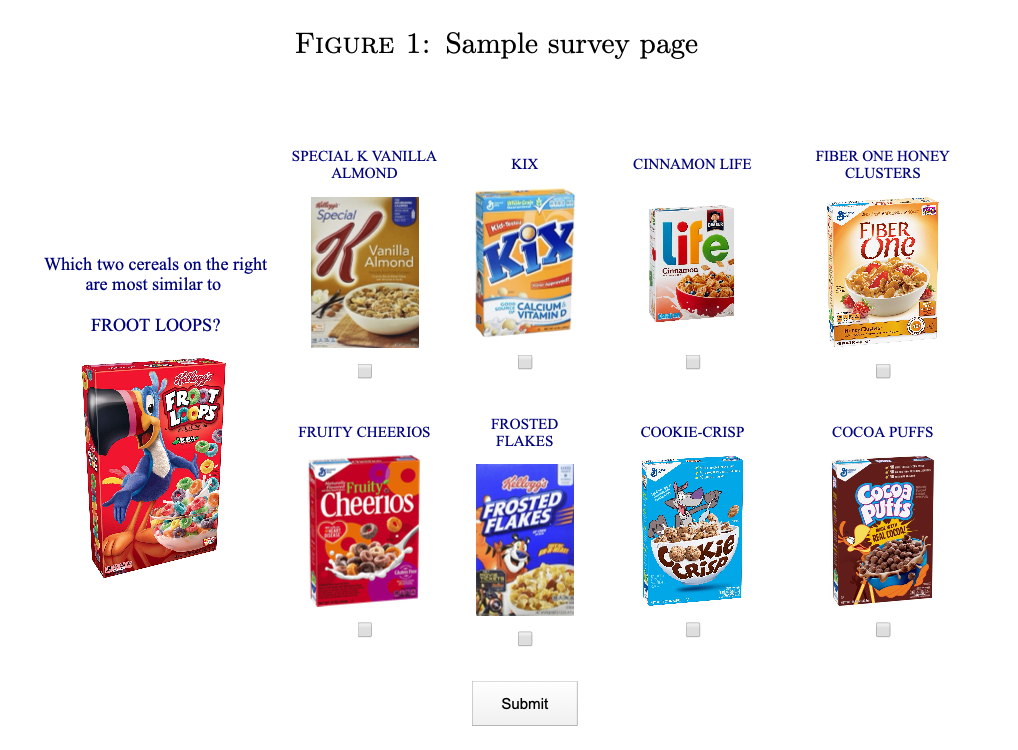
\includegraphics[width=\textwidth]{resources/embeddings_1}      
\end{column}
\begin{column}{0.5\textwidth}
What if we could first estimate \alert{unobserved characteristics}?
\begin{itemize}
    \item Is $j$ more similar to $k$ or $l$?
    \item Use \alert{embedding} procedure to calculate what amounts to a likelihood
\begin{align*}
\max_{\mathbf{X} \in \mathbb{R}^{m \times J}} \ln \left(\frac{f(||x_l - x_j|| ,\alpha)}{f(||x_l - x_j|| ,\alpha)+{f(||x_k - x_j|| ,\alpha)}}\right)
\end{align*}
\item Get a $m \times J$ matrix with $m$ factors (embeddings).
\item Idea: $m$ is small (like 3-4).
\end{itemize}
\end{column}
\end{columns}
\end{frame}

\begin{frame}{Unobserved Characteristics: Magnolfi Maclure Sorensen (2023)}
\begin{columns}
\begin{column}{0.5\textwidth}
     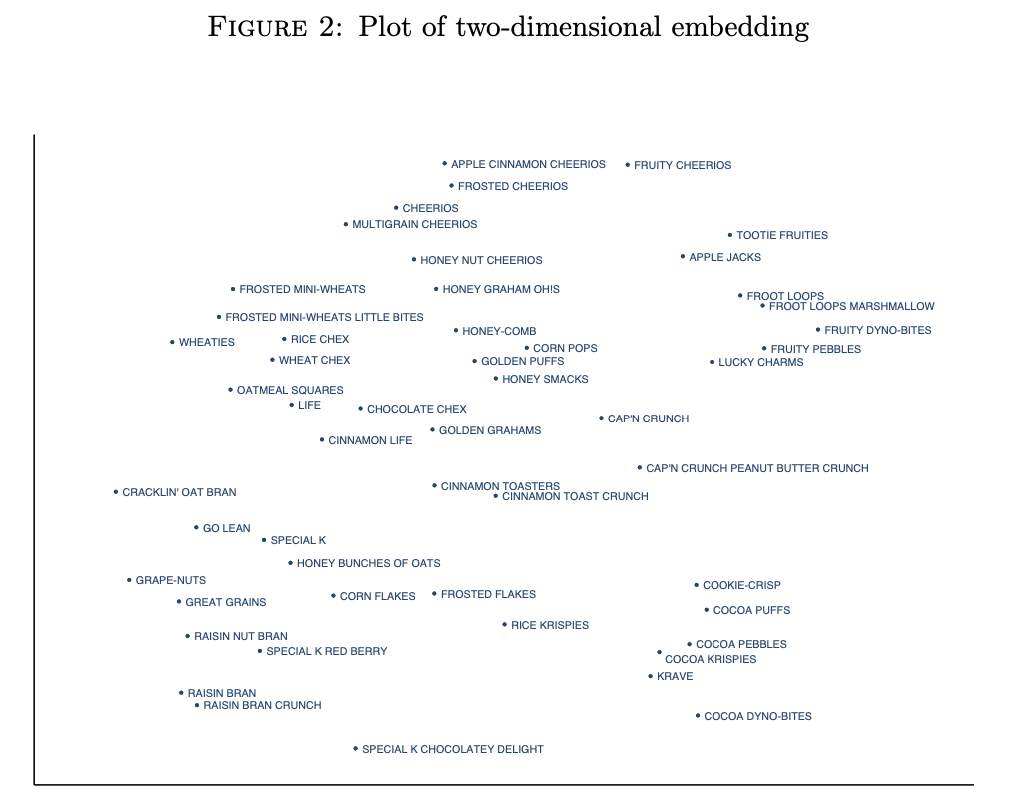
\includegraphics[width=\textwidth]{resources/embeddings_2}      
\end{column}
\begin{column}{0.5\textwidth}
     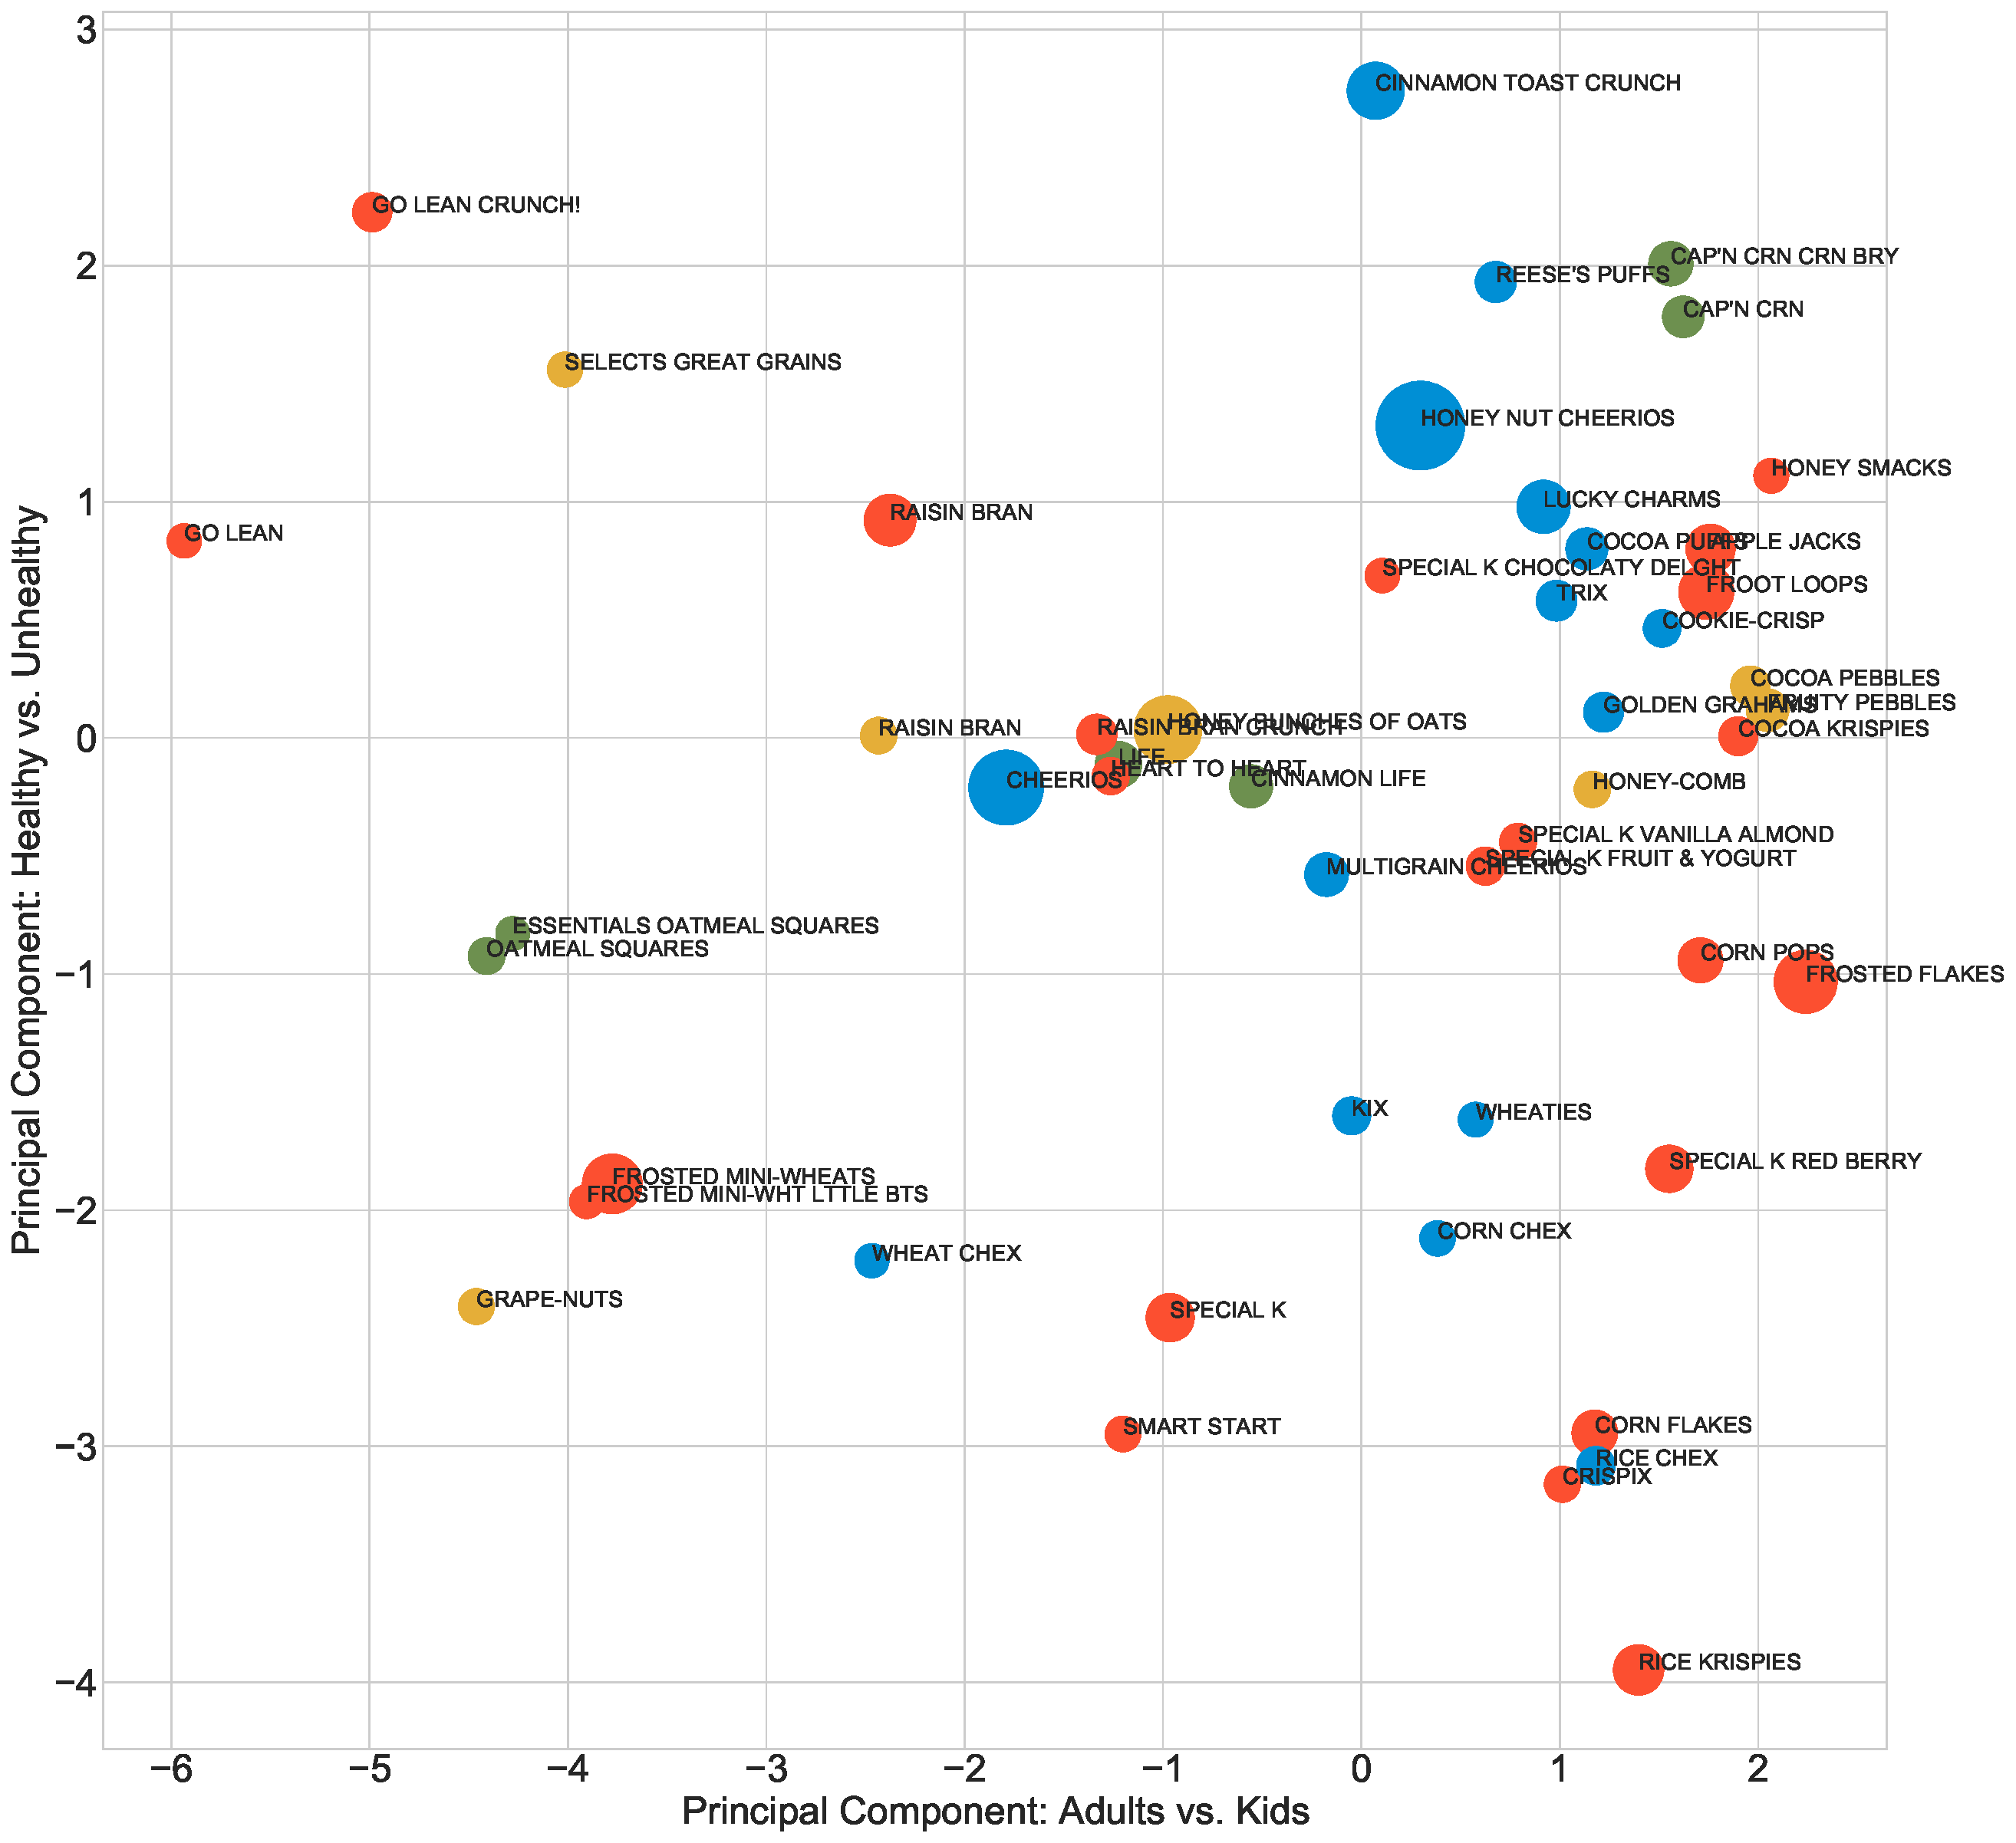
\includegraphics[width=\textwidth]{resources/pca_01}      
\end{column}
\end{columns}
\end{frame}





\begin{frame}{Conlon, Mortimer, Sarkis (2024): Structural Low Rank Approximations}
\small
Fix $\textrm{rank}(\mathbf{D}(\mathbf{S},\pi))=I$, and for each choice of $I$ solve:
\begin{align*}
\min _{(\mathbf{S}, \pi) \geq 0} \left\|\mathcal{P}_{\Omega}(\mathcal{D}-\mathbf{D}(\mathbf{S},\pi))\right\|_{\ell_2}  &+ \lambda \left\|\mathcal{S}- \mathbf{S}\,\pi \right\|_{\ell_2} \text { with } \left\|\pi  \right\|_{\ell_1} \leq 1, \quad   \left\|\mathbf{s_i}  \right\|_{\ell_1} \leq 1.
\end{align*}
\vspace{-.25cm}
\begin{itemize}
\item Goal: estimate $\mathbf{s_i}$ (choice probabilities) and corresponding weights $\pi_i$ (Finite Mixture) in \alert{product space}
\begin{itemize}
\item Consistent with $U_{ij} = V_{ij} + \varepsilon_{ij}$ and logit error.
\end{itemize}
\item Constraints: Choice probabilities $s_{ij}$ sum to one, type weights $\pi_i$ sum to one.
\begin{itemize}
\item $\ell_1$ constraints lead to \alert{sparsity}.
\end{itemize}
\item Idea: \alert{Control the rank by limiting $I$ directly}
\begin{itemize}
\item Use cross validation to select \# of types $I$ and Lagrange multiplier $\lambda$.
\end{itemize}
\item Matrix completion: We can construct estimates of $\mathbf{D}(\mathbf{S},\pi)$ including elements of $\mathcal{P}_{\overline{\Omega}}$.
% \item Weights $\widetilde c_j$ and $c_j$ are proportional to $\ln q_j$
\end{itemize}
\end{frame}

\begin{frame}{In-Sample Performance}
\label{in_sample}
%\hyperlink{cross_valid}{\beamerbutton{Cross Validation}}
\centering
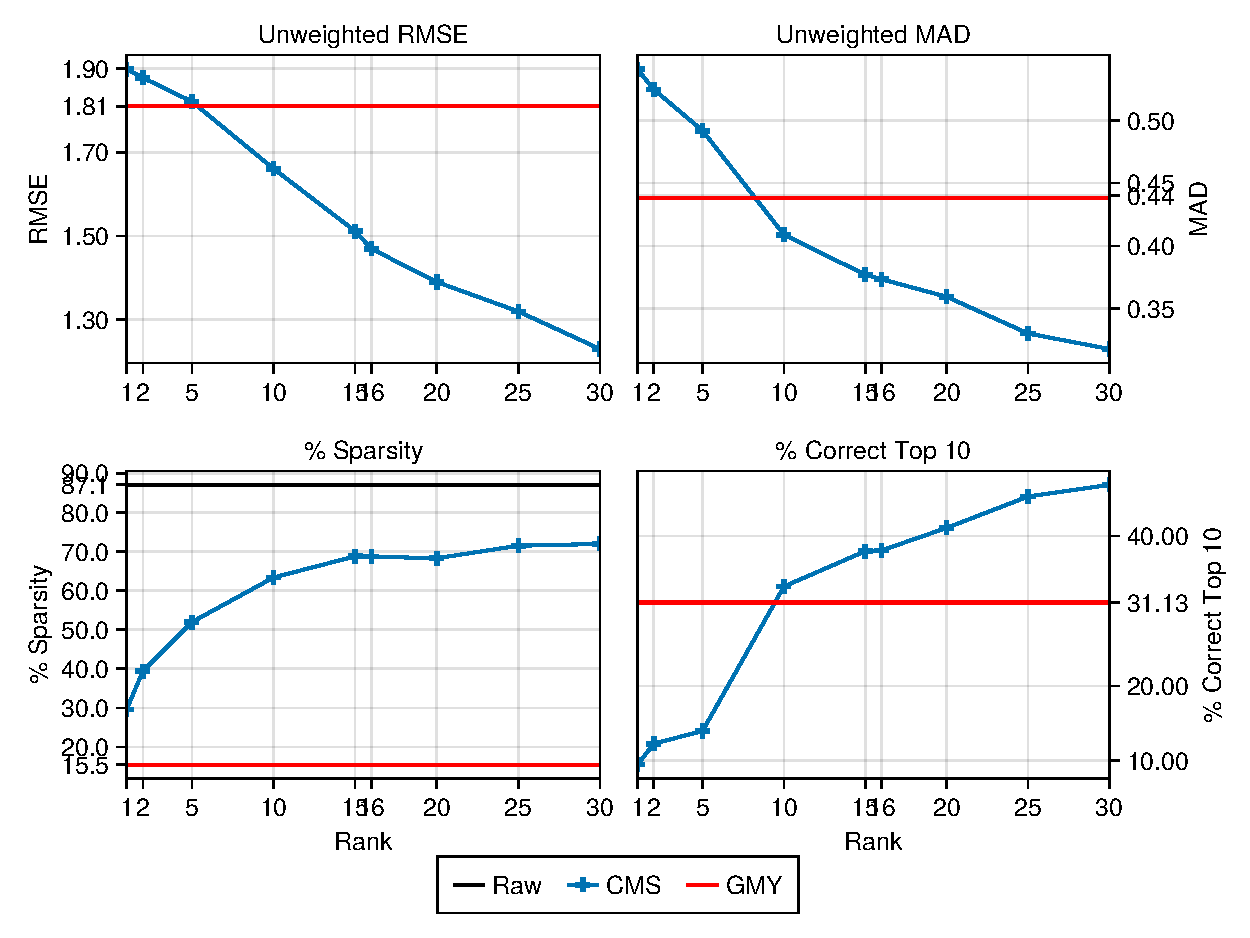
\includegraphics[height=\textheight,width=\textwidth, keepaspectratio]{resources/insample-comparison-all.pdf}\\
\end{frame}


\begin{frame}{Profiles of Types (Rank 15)}
\centering
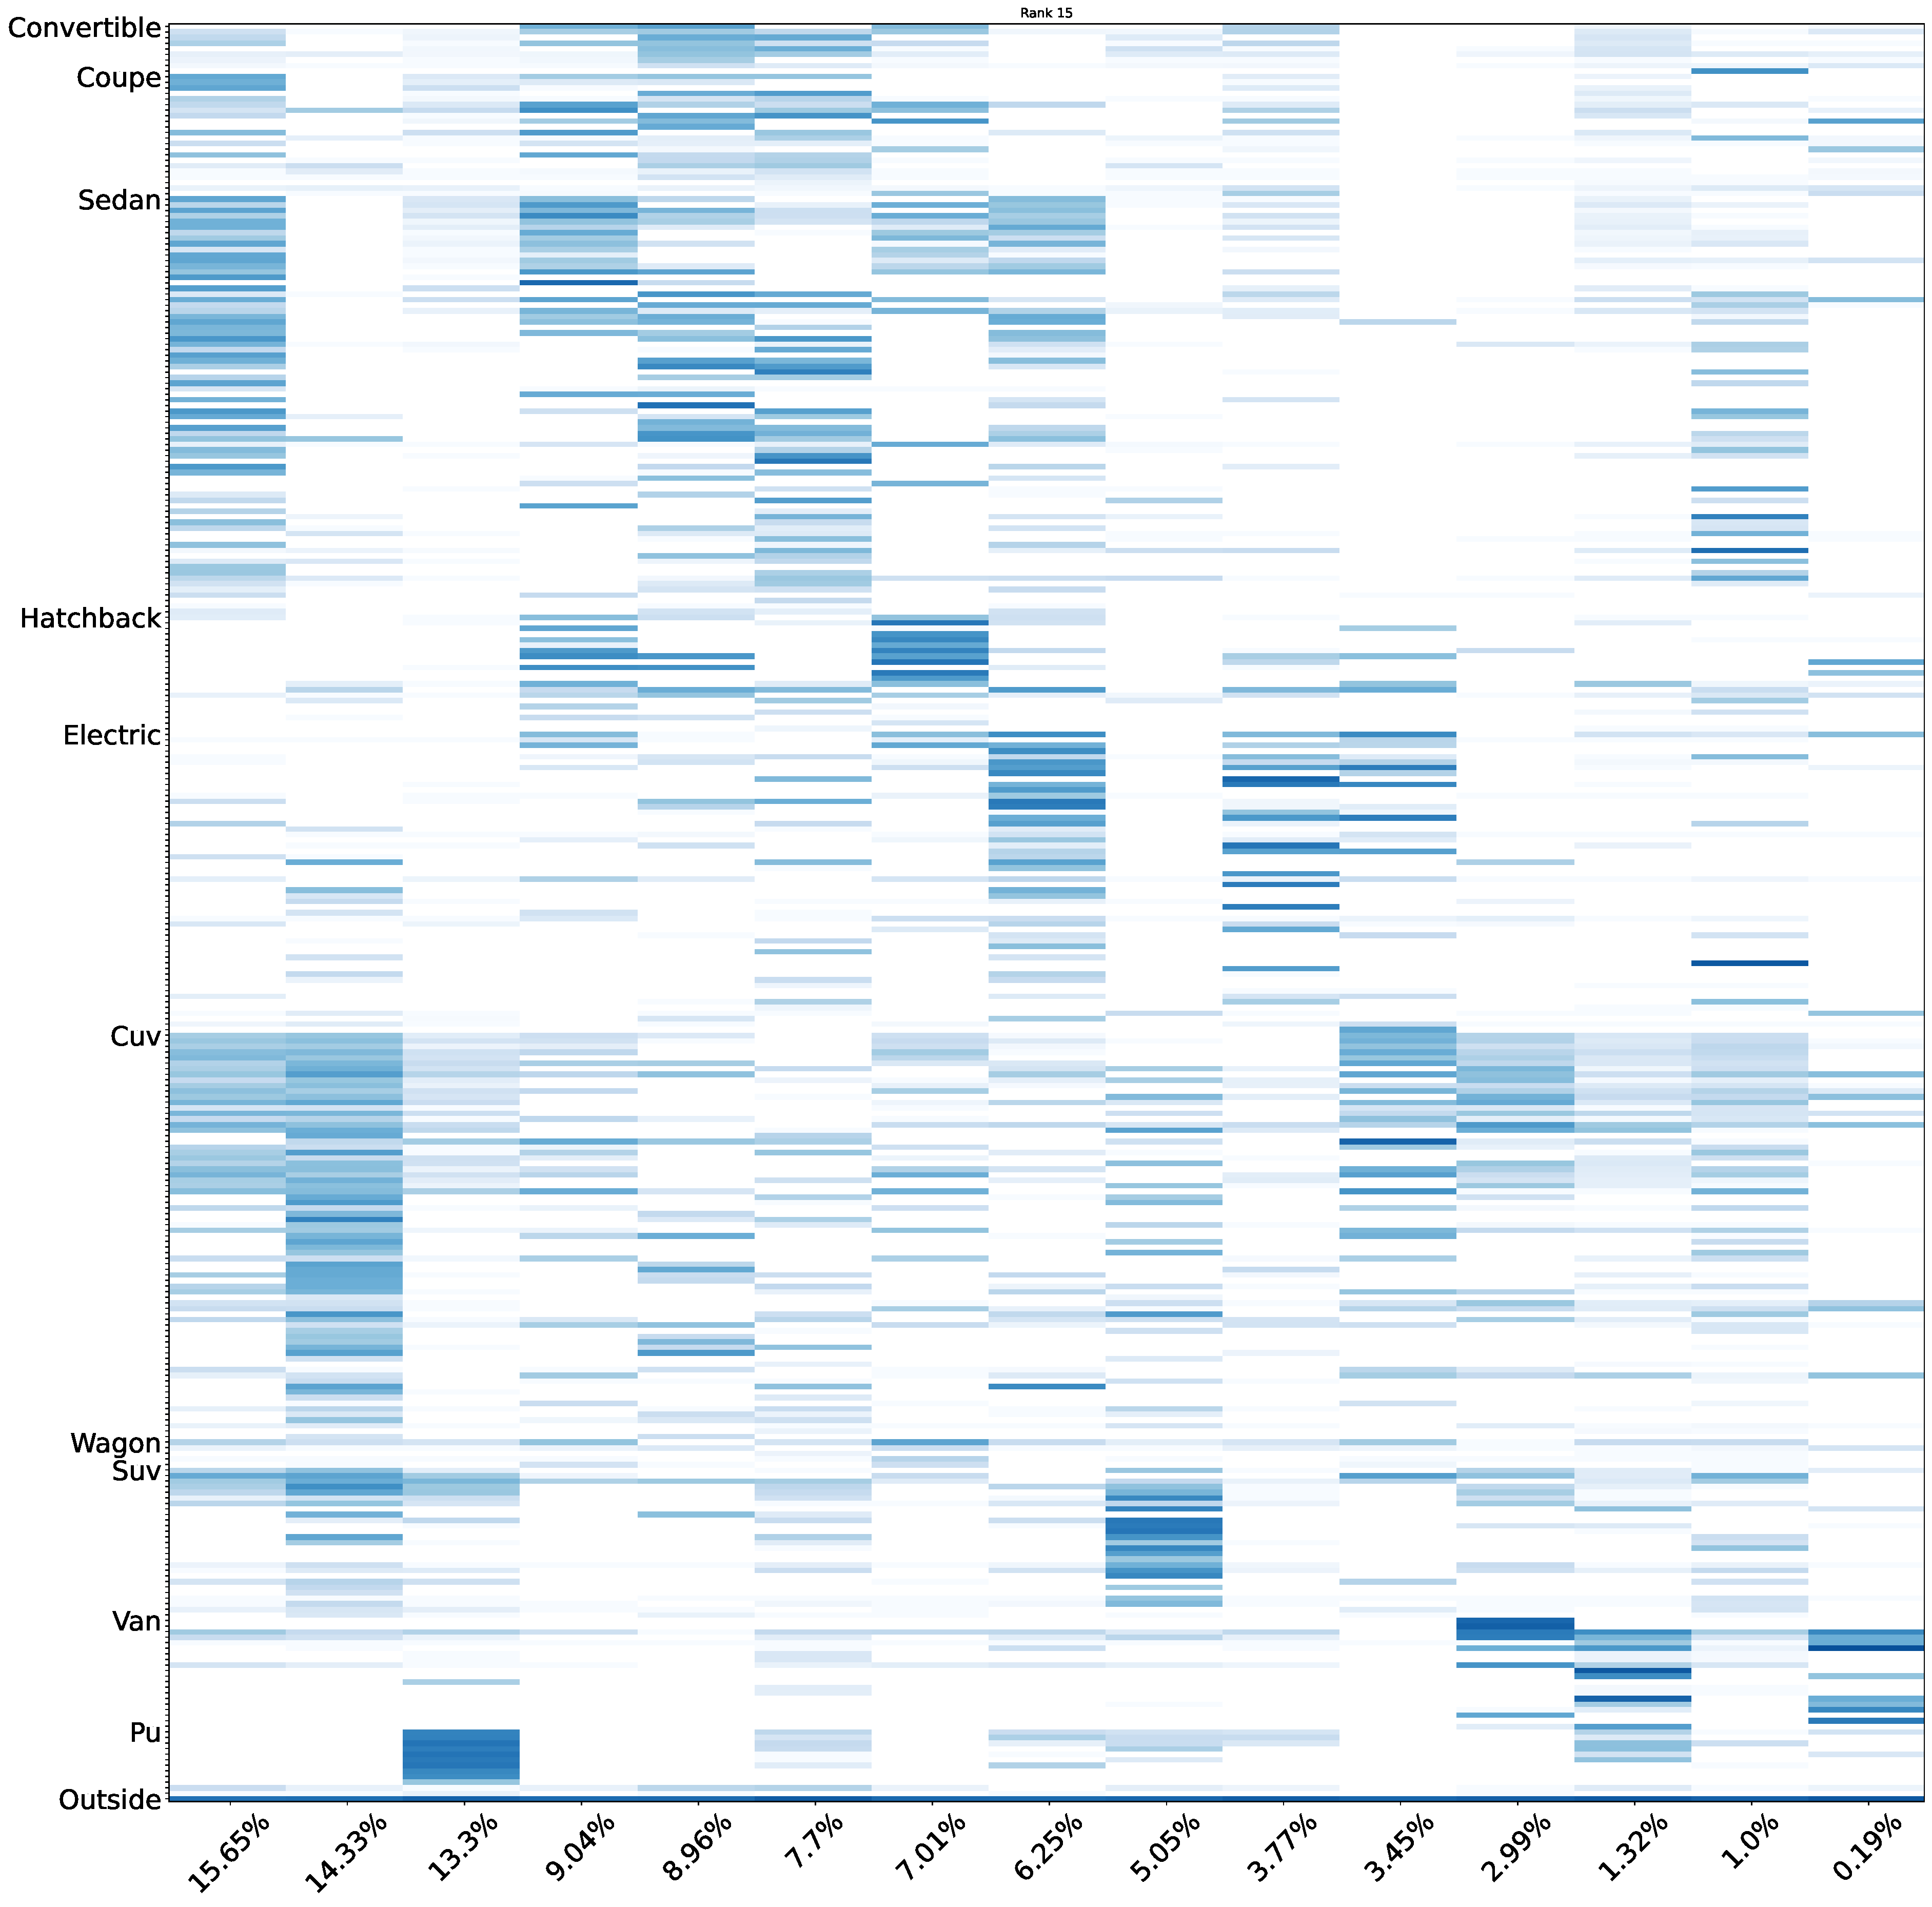
\includegraphics[height=0.95\textheight]{resources/hpc_rank_15_profiles}
\end{frame}

 \begin{frame}{Top Substitutes: Ford F-Series}
    \centering
    \begin{tabular}{rrrrrr}
  \hline
  \textbf{Model} & \textbf{Raw} & \textbf{Logit} & \textbf{CMS I=15} & \textbf{CMS I=30} & \textbf{GMY} \\\hline
  Ram Pickup & 24.59 & 0.88 & 21.46 & 22.23 & 19.4 \\
  Gmc Sierra & 20.29 & 0.61 & 14.97 & 21.92 & 17.27 \\
  Chevrolet Silverado & 15.62 & 0.78 & 13.408 & 19.63 & 33.62 \\
  Toyota Tundra & 12.98 & 0.55 & 16.32 & 12.79 & 2.29 \\
  Toyota Tacoma & 6.31 & 0.76 & 3.39 & 3.13 & 2.83 \\
  Chevrolet Colorado & 4.64 & 0.63 & 3.22 & 2.86 & 2.87 \\
  Gmc Canyon & 2.3 & 0.3 & 0.76 & 1.38 & 1.02 \\
  Nissan Frontier & 1.63 & 0.43 & 0.92 & 1.69 & 0.61 \\
  Jeep Wrangler & 1.59 & 0.69 & 1.33 & 0.94 & 0.06 \\
  Nissan Titan & 0.7 & 0.05 & 1.18 & 1.17 & 0.18 \\
  Ford Explorer & 0.63 & 0.38 & 0.16 & 0.14 & 0.71 \\\hline
\end{tabular}
\\
 \end{frame}


\begin{frame}{}
  \centering \Large
  \emph{Thanks!}\\

  Reach me at cconlon@stern.nyu.edu\\

  Slides at \url{bit.ly/conlon\_IIOC}
\end{frame}


\begin{frame}[plain,allowframebreaks,noframenumbering]{References}
    \bibliography{references}
\end{frame}

\end{document}